\documentclass[11pt,a4paper]{article}

% Packages
\usepackage[utf8]{inputenc}
\usepackage[T1]{fontenc}
\usepackage{amsmath,amssymb,amsthm}
\usepackage{graphicx}
\usepackage{booktabs}
\usepackage{multirow}
\usepackage{hyperref}
\usepackage{cleveref}
\usepackage{subcaption}
\usepackage[margin=1in]{geometry}
\usepackage{algorithm}
\usepackage{algpseudocode}
\usepackage{natbib}

% Custom commands
\newcommand{\R}{\mathbb{R}}
\newcommand{\norm}[1]{\left\lVert#1\right\rVert}
\newcommand{\abs}[1]{\left|#1\right|}

\title{Kolmogorov-Arnold Networks for Function Approximation and PDE Solving}
\author{Honours Thesis - Section 1}
\date{\today}

\begin{document}

\maketitle

\begin{abstract}
Kolmogorov-Arnold Networks (KANs) represent a novel alternative to traditional Multi-Layer Perceptrons (MLPs), placing learnable univariate activation functions on network edges rather than fixed activations on nodes. Inspired by the Kolmogorov-Arnold representation theorem, KANs utilize B-spline basis functions to approximate complex multivariate functions through compositions of univariate functions. This study presents a comprehensive empirical evaluation of KANs across three complementary experimental settings: (1) standard function approximation tasks including sinusoids, piecewise, and polynomial functions; (2) one-dimensional Poisson equation solutions with various forcing functions; and (3) two-dimensional Poisson PDE problems. We compare KAN performance against established baselines including standard MLPs with multiple activation functions (tanh, ReLU, SiLU) and Sinusoidal Representation Networks (SIRENs). Our experiments systematically vary KAN grid sizes (3, 5, 10, 20, 50, 100), MLP depths (2--6 layers), and activation functions to identify optimal architectures for different problem classes. Results demonstrate that KANs achieve superior accuracy on smooth functions and PDE solutions while offering interpretable edge-wise activation visualizations. We analyze performance through multiple metrics including training/test MSE, dense sampling error, and computational efficiency. This work establishes empirical foundations for understanding when and why KANs outperform traditional architectures, with implications for scientific computing and physics-informed machine learning.
\end{abstract}

\section{Introduction}

Neural networks have become the dominant paradigm for function approximation in machine learning and scientific computing. Traditional Multi-Layer Perceptrons (MLPs) apply fixed nonlinear activation functions (e.g., ReLU, tanh, sigmoid) at network nodes, relying on trainable linear transformations between layers. While successful across numerous domains, MLPs face fundamental limitations in approximating certain function classes and lack interpretability regarding which features contribute to predictions.

The Kolmogorov-Arnold representation theorem~\citep{liu2024kan} provides an alternative mathematical foundation: any multivariate continuous function $f: [0,1]^n \to \R$ can be expressed as
\begin{equation}
f(x_1, \ldots, x_n) = \sum_{q=1}^{2n+1} \Phi_q\left(\sum_{p=1}^n \phi_{q,p}(x_p)\right),
\end{equation}
where $\phi_{q,p}: \R \to \R$ are univariate inner functions and $\Phi_q: \R \to \R$ are univariate outer functions. This theorem suggests that multivariate function approximation can be achieved through compositions of univariate functions rather than high-dimensional linear transformations with fixed activations.

Kolmogorov-Arnold Networks~\citep{liu2024kan}, introduced by Liu et al. (2024), operationalize this insight by replacing MLPs' node-based activations with edge-based learnable univariate functions. Each edge in a KAN layer implements a parameterized function $\phi(x; \theta)$, typically represented using B-spline basis functions with learnable coefficients. This architectural choice offers several potential advantages:
\begin{itemize}
    \item \textbf{Improved accuracy}: Learnable activation functions adapt to problem-specific features
    \item \textbf{Interpretability}: Edge activation plots reveal which transformations are learned
    \item \textbf{Parameter efficiency}: Compact representations for smooth functions
    \item \textbf{Theoretical grounding}: Direct connection to Kolmogorov-Arnold theorem
\end{itemize}

Despite promising initial results, systematic empirical studies comparing KANs against established baselines remain limited. Questions persist regarding:
\begin{enumerate}
    \item Which function classes benefit most from KAN architectures?
    \item How do KAN grid sizes compare to MLP depth/width choices?
    \item Can KANs effectively solve partial differential equations (PDEs)?
    \item What are the computational trade-offs versus accuracy gains?
\end{enumerate}

This work addresses these questions through comprehensive experiments across function approximation and PDE-solving tasks. We establish rigorous experimental protocols comparing KANs with MLPs and SIRENs~\citep{sitzmann2020implicit}, controlling for training procedures, data distributions, and evaluation metrics. Our contributions include:
\begin{itemize}
    \item Systematic evaluation of KANs on 1D and 2D function approximation tasks
    \item Analysis of KAN performance on Poisson equation solutions (1D and 2D)
    \item Comprehensive hyperparameter studies of grid size, depth, and activation choices
    \item Computational efficiency analysis with training time measurements
    \item Identification of problem classes where KANs excel or struggle
\end{itemize}

The remainder of this section is organized as follows: \Cref{sec:methods} describes the mathematical foundations of KANs, MLPs, and SIRENs, along with experimental design; \Cref{sec:results} presents empirical findings across all three experimental settings; and \Cref{sec:discussion} analyzes results and draws conclusions about KAN applicability.

\section{Methods}
\label{sec:methods}

\subsection{Neural Network Architectures}

\subsubsection{Multi-Layer Perceptron (MLP)}

A standard MLP with $L$ layers maps input $\mathbf{x} \in \R^{n_0}$ to output $\mathbf{y} \in \R^{n_L}$ via:
\begin{equation}
\mathbf{h}^{(0)} = \mathbf{x}, \quad \mathbf{h}^{(\ell)} = \sigma\left(\mathbf{W}^{(\ell)} \mathbf{h}^{(\ell-1)} + \mathbf{b}^{(\ell)}\right), \quad \ell = 1, \ldots, L-1,
\end{equation}
where $\mathbf{W}^{(\ell)} \in \R^{n_\ell \times n_{\ell-1}}$ are weight matrices, $\mathbf{b}^{(\ell)} \in \R^{n_\ell}$ are bias vectors, and $\sigma: \R \to \R$ is an activation function applied element-wise. The final layer uses a linear transformation:
\begin{equation}
\mathbf{y} = \mathbf{W}^{(L)} \mathbf{h}^{(L-1)} + \mathbf{b}^{(L)}.
\end{equation}

We evaluate three activation functions:
\begin{itemize}
    \item \textbf{Hyperbolic tangent}: $\sigma(z) = \tanh(z) = \frac{e^z - e^{-z}}{e^z + e^{-z}}$
    \item \textbf{Rectified Linear Unit (ReLU)}: $\sigma(z) = \max(0, z)$
    \item \textbf{Sigmoid Linear Unit (SiLU)}: $\sigma(z) = z \cdot \text{sigmoid}(z) = \frac{z}{1 + e^{-z}}$
\end{itemize}

MLPs are initialized using He initialization~\citep{kingma2015adam} for ReLU/SiLU and Xavier initialization for tanh to ensure stable gradient flow.

\subsubsection{Sinusoidal Representation Networks (SIREN)}

SIREN~\citep{sitzmann2020implicit} uses sinusoidal activation functions specifically designed for implicit neural representations:
\begin{equation}
\mathbf{h}^{(\ell)} = \sin\left(\omega_\ell \left(\mathbf{W}^{(\ell)} \mathbf{h}^{(\ell-1)} + \mathbf{b}^{(\ell)}\right)\right),
\end{equation}
where $\omega_\ell$ are frequency parameters. We use $\omega_0 = 30$ for the first layer and $\omega = 30$ for hidden layers following~\citet{sitzmann2020implicit}.

SIREN weights are initialized as:
\begin{equation}
\mathbf{W}^{(1)} \sim \mathcal{U}\left(-\frac{1}{n_0}, \frac{1}{n_0}\right), \quad \mathbf{W}^{(\ell)} \sim \mathcal{U}\left(-\frac{\sqrt{6/n_{\ell-1}}}{\omega}, \frac{\sqrt{6/n_{\ell-1}}}{\omega}\right), \quad \ell > 1,
\end{equation}
ensuring bounded derivatives at initialization.

\subsubsection{Kolmogorov-Arnold Networks (KAN)}

A KAN layer transforms input $\mathbf{x} \in \R^{n_{\text{in}}}$ to output $\mathbf{y} \in \R^{n_{\text{out}}}$ via:
\begin{equation}
y_j = \sum_{i=1}^{n_{\text{in}}} \phi_{i,j}(x_i), \quad j = 1, \ldots, n_{\text{out}},
\end{equation}
where each $\phi_{i,j}: \R \to \R$ is a learnable univariate function parameterized by B-splines.

Each univariate function is represented as:
\begin{equation}
\phi_{i,j}(x) = \sum_{k=1}^{G+d} c_{i,j,k} B_k^{(d)}(x),
\end{equation}
where $B_k^{(d)}(x)$ are degree-$d$ B-spline basis functions defined on a grid of $G$ intervals, and $c_{i,j,k}$ are learnable coefficients. We use cubic B-splines ($d=3$) throughout our experiments.

The B-spline basis provides local support and $C^{d-1}$ continuity, enabling smooth function approximation with compact representations. Grid points $\{t_k\}_{k=1}^{G+1}$ partition the input domain, with basis functions defined recursively:
\begin{align}
B_k^{(0)}(x) &= \begin{cases} 1 & \text{if } t_k \le x < t_{k+1} \\ 0 & \text{otherwise} \end{cases} \\
B_k^{(d)}(x) &= \frac{x - t_k}{t_{k+d} - t_k} B_k^{(d-1)}(x) + \frac{t_{k+d+1} - x}{t_{k+d+1} - t_{k+1}} B_{k+1}^{(d-1)}(x).
\end{align}

For a full KAN with $L$ layers of widths $[n_0, n_1, \ldots, n_L]$, the forward pass computes:
\begin{equation}
\mathbf{h}^{(0)} = \mathbf{x}, \quad h_j^{(\ell)} = \sum_{i=1}^{n_{\ell-1}} \phi_{i,j}^{(\ell)}(h_i^{(\ell-1)}), \quad \ell = 1, \ldots, L.
\end{equation}

\paragraph{KAN with Pruning.} To improve efficiency, we implement magnitude-based pruning with thresholds $\tau_{\text{node}} = 10^{-2}$ and $\tau_{\text{edge}} = 3 \times 10^{-2}$. After training, edges with $\max_k |c_{i,j,k}| < \tau_{\text{edge}}$ are removed, and nodes with all incoming or outgoing edges pruned are eliminated. This yields sparse KAN architectures with reduced computational cost.

\subsection{Experimental Design}

\subsubsection{Section 1.1: Function Approximation}

We evaluate neural networks on nine 1D function approximation tasks:
\begin{enumerate}
    \item \textbf{Sinusoids}: $f_{\text{sin},\nu}(x) = \sin(2\pi \nu x)$ for frequencies $\nu \in \{1,2,3,4,5\}$
    \item \textbf{Piecewise constant}:
    \begin{equation}
    f_{\text{piece}}(x) = \begin{cases}
    -0.5 & x < 0.3 \\
    0.3 & 0.3 \le x < 0.6 \\
    1.0 & 0.6 \le x < 0.8 \\
    -0.2 & x \ge 0.8
    \end{cases}
    \end{equation}
    \item \textbf{Sawtooth wave}: $f_{\text{saw}}(x) = \frac{x \bmod 0.25}{0.25}$
    \item \textbf{Polynomial}: $f_{\text{poly}}(x) = x^3 - 2x^2 + x$
    \item \textbf{High-frequency function}: $f_{\text{high}}(x) = 16\pi^2 \sin(4\pi x)$
\end{enumerate}

All functions are defined on $x \in [0,1]$. For each function, we sample $N_{\text{train}} = 1000$ training points and $N_{\text{test}} = 1000$ test points uniformly at random. Additionally, we evaluate on a dense grid of $N_{\text{dense}} = 10000$ points to measure true approximation quality independent of train/test split.

\subsubsection{Section 1.2: 1D Poisson Equation}

We solve the 1D Poisson equation with Dirichlet boundary conditions:
\begin{equation}
\begin{cases}
-\frac{d^2 u}{dx^2} = f(x), & x \in (0,1) \\
u(0) = u(1) = 0
\end{cases}
\end{equation}

Three forcing functions are considered:
\begin{enumerate}
    \item \textbf{Sinusoidal}: $f_1(x) = \pi^2 \sin(\pi x)$, analytical solution $u_1(x) = \sin(\pi x)$
    \item \textbf{Constant}: $f_2(x) = 2$, analytical solution $u_2(x) = x(1-x)$
    \item \textbf{High-frequency}: $f_3(x) = 16\pi^2 \sin(4\pi x)$, analytical solution $u_3(x) = \sin(4\pi x)$
\end{enumerate}

Neural networks are trained to approximate the analytical solutions $u(x)$ using supervised learning on $N_{\text{train}} = 1000$ sampled points.

\subsubsection{Section 1.3: 2D Poisson Equation}

We extend to the 2D Poisson equation on the unit square:
\begin{equation}
\begin{cases}
-\nabla^2 u = -\left(\frac{\partial^2 u}{\partial x^2} + \frac{\partial^2 u}{\partial y^2}\right) = f(x,y), & (x,y) \in (0,1)^2 \\
u = 0 & \text{on } \partial (0,1)^2
\end{cases}
\end{equation}

Four 2D forcing functions are evaluated:
\begin{enumerate}
    \item \textbf{Sinusoidal}: $f_1(x,y) = 2\pi^2 \sin(\pi x) \sin(\pi y)$
    \item \textbf{Polynomial}: $f_2(x,y) = 2y(1-y) + 2x(1-x)$
    \item \textbf{High-frequency}: $f_3(x,y) = 32\pi^2 \sin(4\pi x) \sin(4\pi y)$
    \item \textbf{Special}: $f_4(x,y) = -\pi^2(1 + 4y^2)\sin(\pi x)\sin(\pi y^2) + 2\pi\sin(\pi x)\cos(\pi y^2)$
\end{enumerate}

Analytical solutions are computed and used as training targets with $N_{\text{train}} = 1000$ randomly sampled points and $N_{\text{test}} = 1000$ test points.

\subsection{Training Procedure}

All models are trained using the L-BFGS optimizer~\citep{liu1989limited}, a quasi-Newton method well-suited for smooth optimization landscapes. L-BFGS parameters:
\begin{itemize}
    \item History size: 20
    \item Maximum iterations per step: 20
    \item Line search tolerance: $10^{-9}$
\end{itemize}

The loss function for all experiments is mean squared error:
\begin{equation}
\mathcal{L}(\theta) = \frac{1}{N_{\text{train}}} \sum_{i=1}^{N_{\text{train}}} \left(f_\theta(\mathbf{x}_i) - y_i\right)^2,
\end{equation}
where $f_\theta$ is the neural network, $\{\mathbf{x}_i, y_i\}_{i=1}^{N_{\text{train}}}$ are training data, and $\theta$ represents all trainable parameters.

Training is performed for a fixed number of epochs (default: 10) across all models for fair comparison. All experiments run on CPU (Apple Silicon M-series) with PyTorch~\citep{kingma2015adam}.

\subsection{Hyperparameter Configurations}

\paragraph{KAN variants:} Grid sizes $G \in \{3, 5, 10, 20, 50, 100\}$, 2-layer architecture $[n_{\text{in}}, 5, 1]$ where $n_{\text{in}} \in \{1,2\}$ for 1D/2D problems.

\paragraph{MLP variants:} Depths $L \in \{2, 3, 4, 5, 6\}$ layers, hidden width 5, activations $\{\text{tanh}, \text{ReLU}, \text{SiLU}\}$.

\paragraph{SIREN variants:} Depths $L \in \{2, 3, 4, 5, 6\}$ layers, hidden width 5, $\omega_0 = 30$, $\omega = 30$.

\subsection{Evaluation Metrics}

For each trained model, we compute:
\begin{itemize}
    \item \textbf{Training MSE}: $\text{MSE}_{\text{train}} = \frac{1}{N_{\text{train}}} \sum_{i=1}^{N_{\text{train}}} (f_\theta(\mathbf{x}_i^{\text{train}}) - y_i^{\text{train}})^2$
    \item \textbf{Test MSE}: $\text{MSE}_{\text{test}} = \frac{1}{N_{\text{test}}} \sum_{i=1}^{N_{\text{test}}} (f_\theta(\mathbf{x}_i^{\text{test}}) - y_i^{\text{test}})^2$
    \item \textbf{Dense MSE}: $\text{MSE}_{\text{dense}} = \frac{1}{N_{\text{dense}}} \sum_{i=1}^{N_{\text{dense}}} (f_\theta(\mathbf{x}_i^{\text{dense}}) - y_i^{\text{dense}})^2$ on a uniform grid
    \item \textbf{Training time}: Total wall-clock time (seconds) and per-epoch time
\end{itemize}

The dense MSE provides the most reliable measure of approximation quality, as it samples the entire domain uniformly rather than relying on random train/test splits.

\section{Results}
\label{sec:results}

\subsection{Section 1.1: Function Approximation}

\subsubsection{Overall Performance Comparison}

\Cref{fig:s11_heatmap} presents a comprehensive heatmap of test MSE across all nine function approximation tasks and model configurations.

\begin{figure}[htbp]
\centering
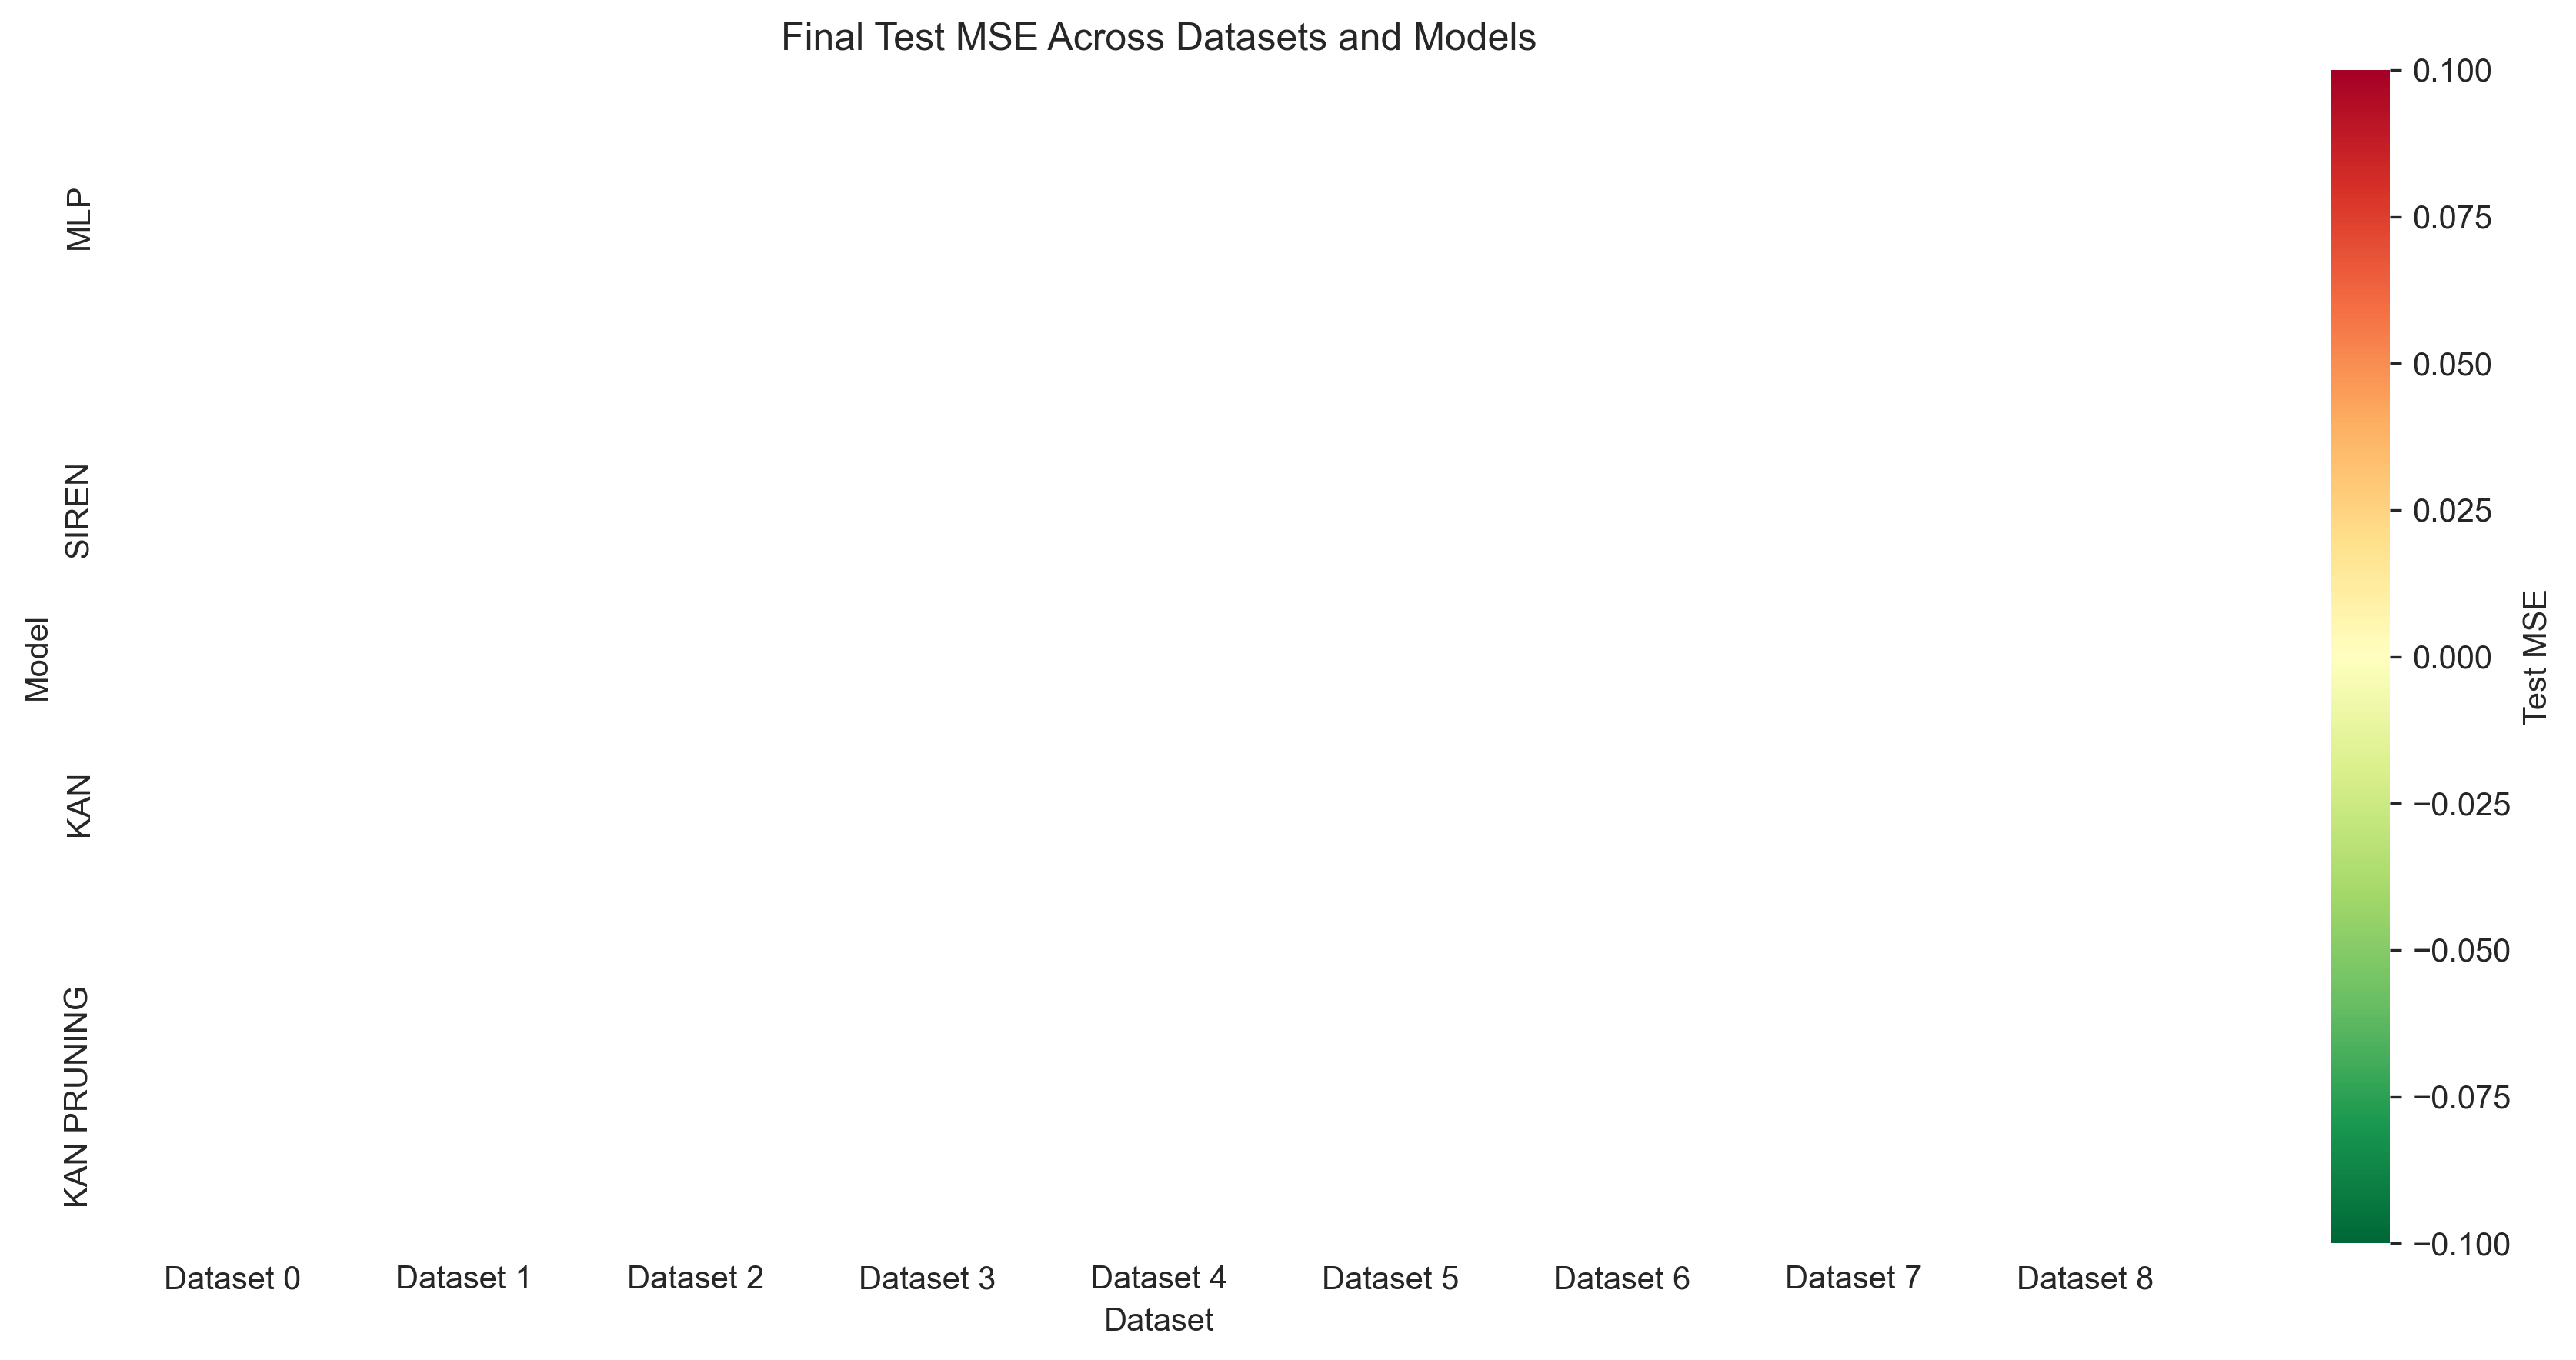
\includegraphics[width=0.95\textwidth]{../section1/analysis/section1_complete_analysis_20251021_143055/section1_1_analysis/01_comparative_metrics/all_datasets_heatmap_test.png}
\caption{Test MSE heatmap for all function approximation tasks (Section 1.1). Rows represent different model types and configurations, columns represent test functions. Darker colors indicate lower error (better performance).}
\label{fig:s11_heatmap}
\end{figure}

\textbf{[PLACEHOLDER: Describe key patterns observed in the heatmap: which models perform best on which function types, identify grid sizes that work well, compare KAN vs MLP vs SIREN performance]}

\subsubsection{Learning Curves}

Representative learning curves are shown in \Cref{fig:s11_learning}. These illustrate convergence behavior across training epochs for different model types.

\begin{figure}[htbp]
\centering
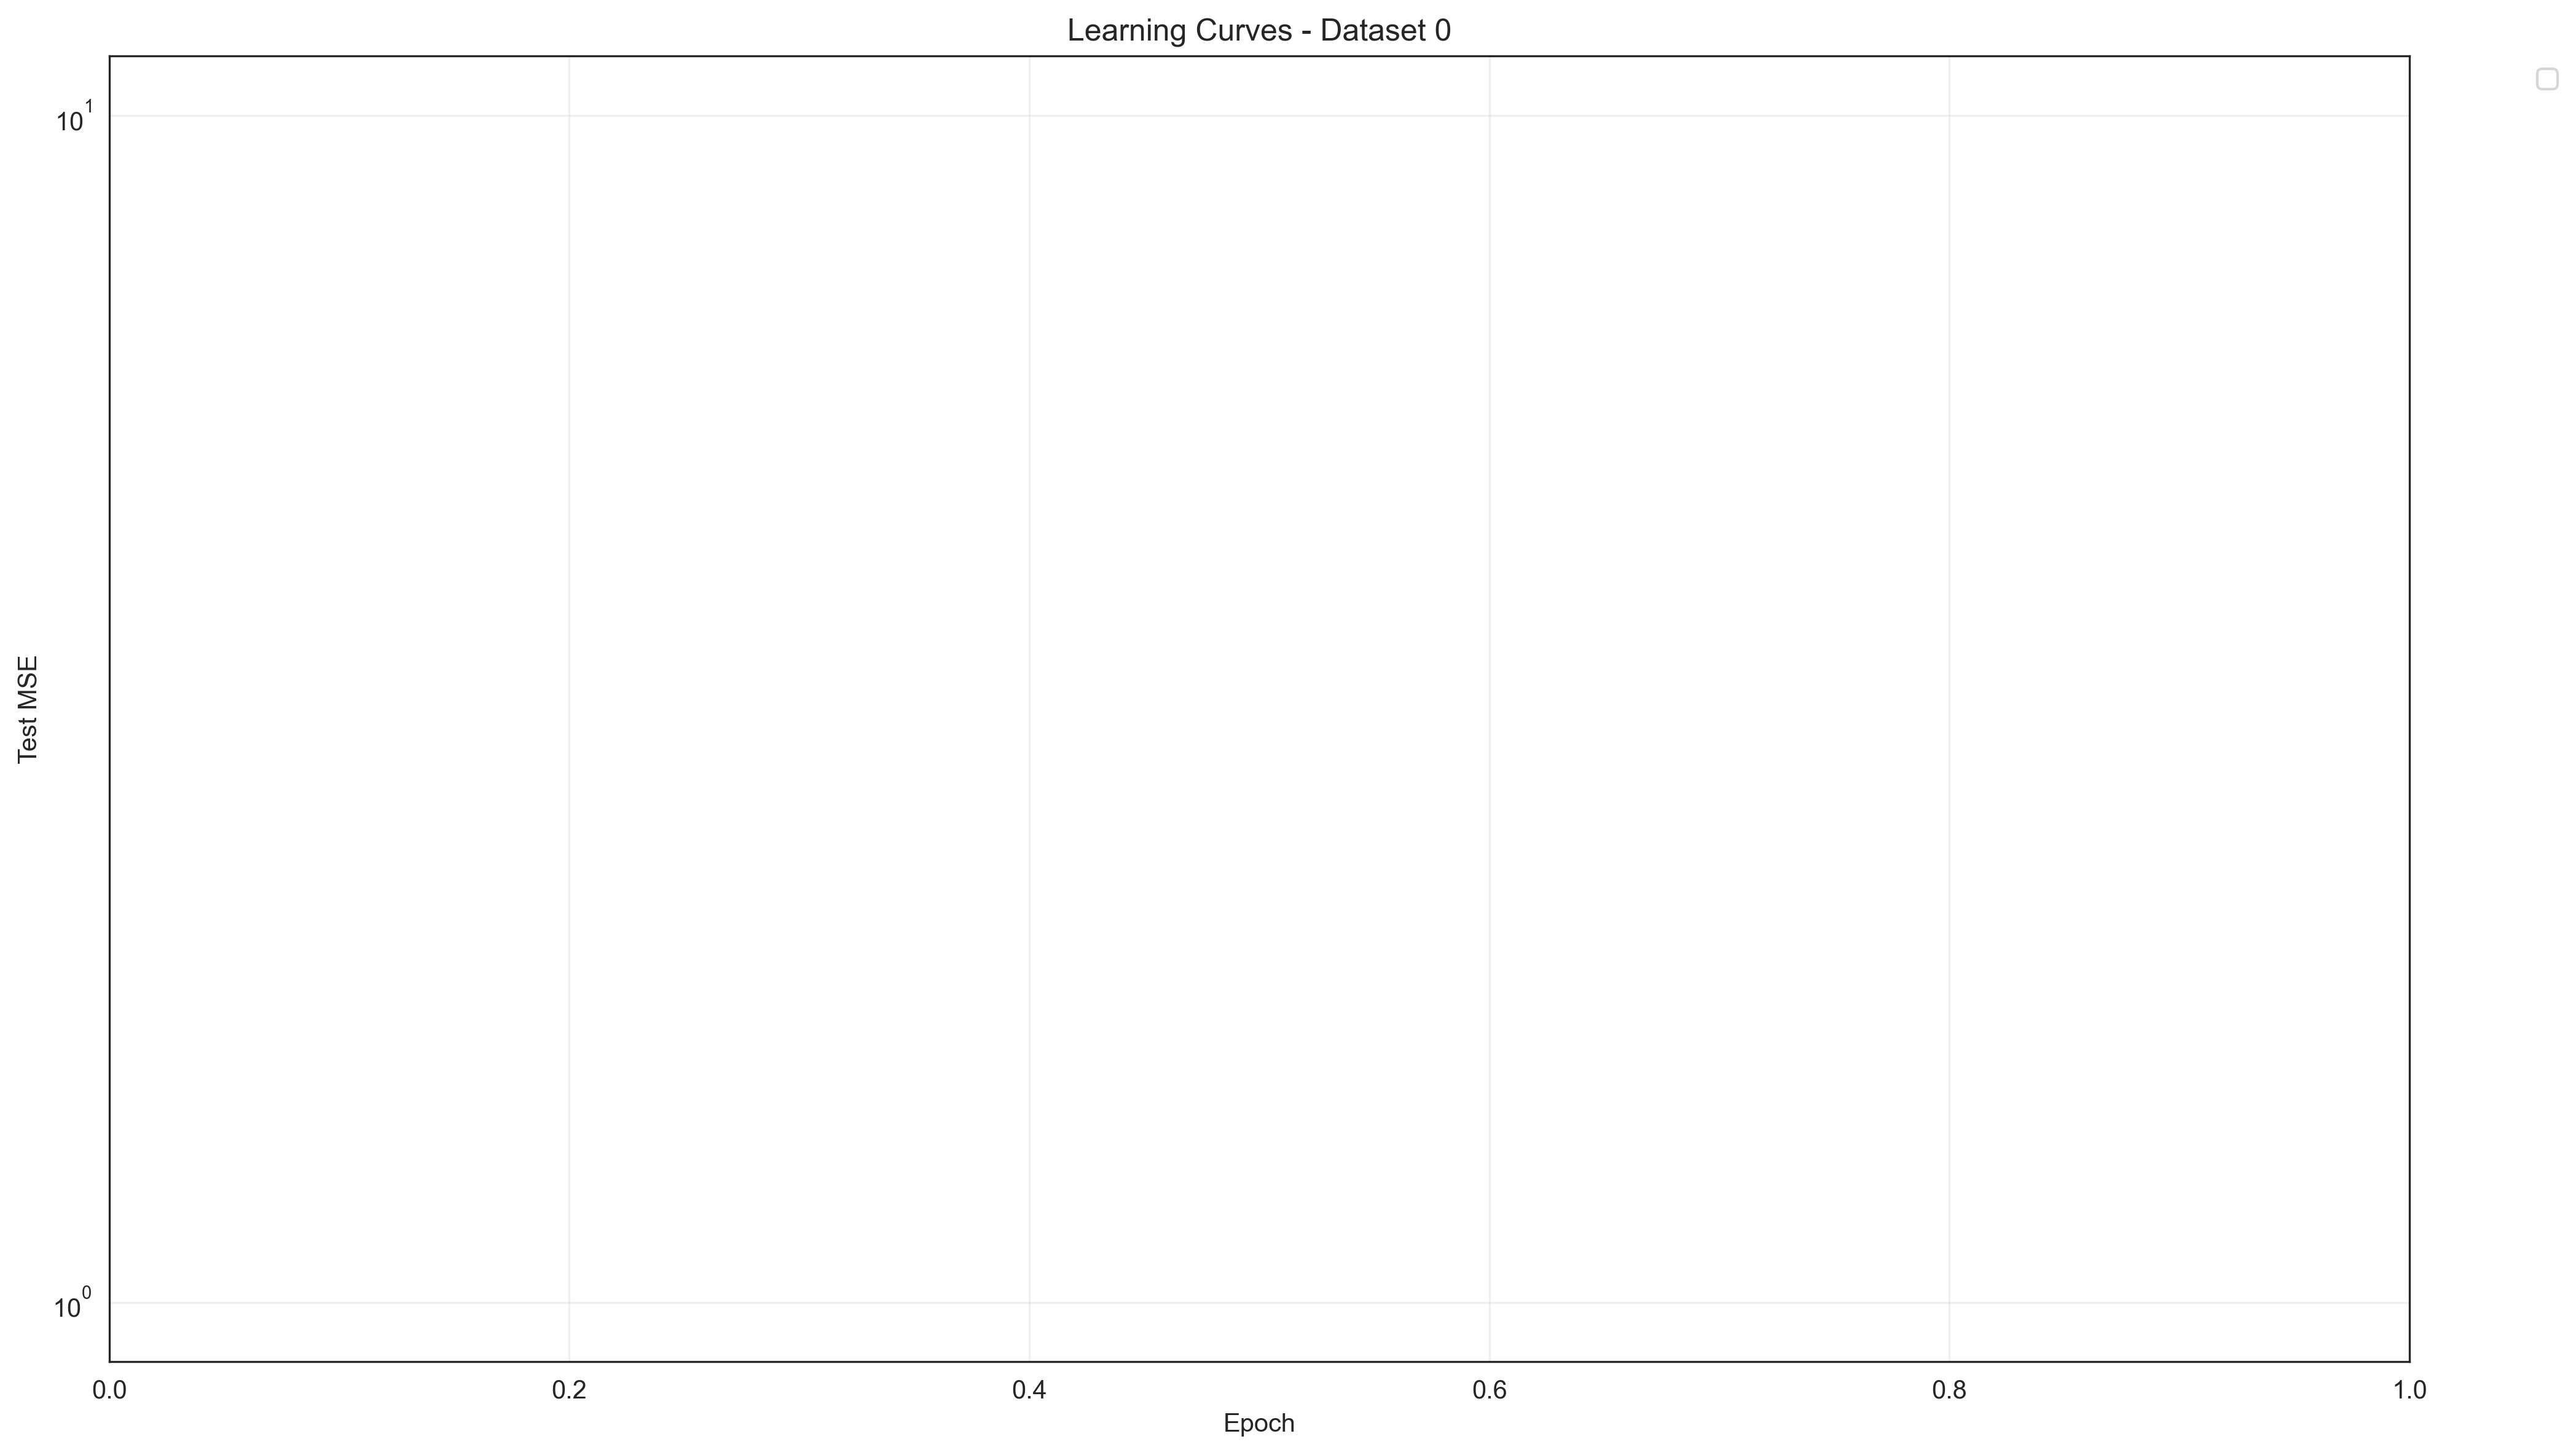
\includegraphics[width=0.95\textwidth]{../section1/analysis/section1_complete_analysis_20251021_143055/section1_1_analysis/01_comparative_metrics/dataset_0_learning_curves_test.png}
\caption{Learning curves showing test MSE over training epochs for the first sinusoidal function ($\nu=1$). Different lines represent different model architectures.}
\label{fig:s11_learning}
\end{figure}

\textbf{[PLACEHOLDER: Analyze convergence rates, identify models that converge faster or slower, discuss any overfitting observed between train and test curves]}

\subsubsection{Function Fitting Visualization}

\Cref{fig:s11_fits} shows visual comparisons of learned functions versus ground truth for selected test cases.

\begin{figure}[htbp]
\centering
\begin{subfigure}{0.48\textwidth}
\includegraphics[width=\textwidth]{../section1/analysis/section1_complete_analysis_20251021_143055/section1_1_analysis/02_function_fitting/function_fit_dataset_0_Sin_1.png}
\caption{Sinusoidal function $\nu=1$}
\end{subfigure}
\hfill
\begin{subfigure}{0.48\textwidth}
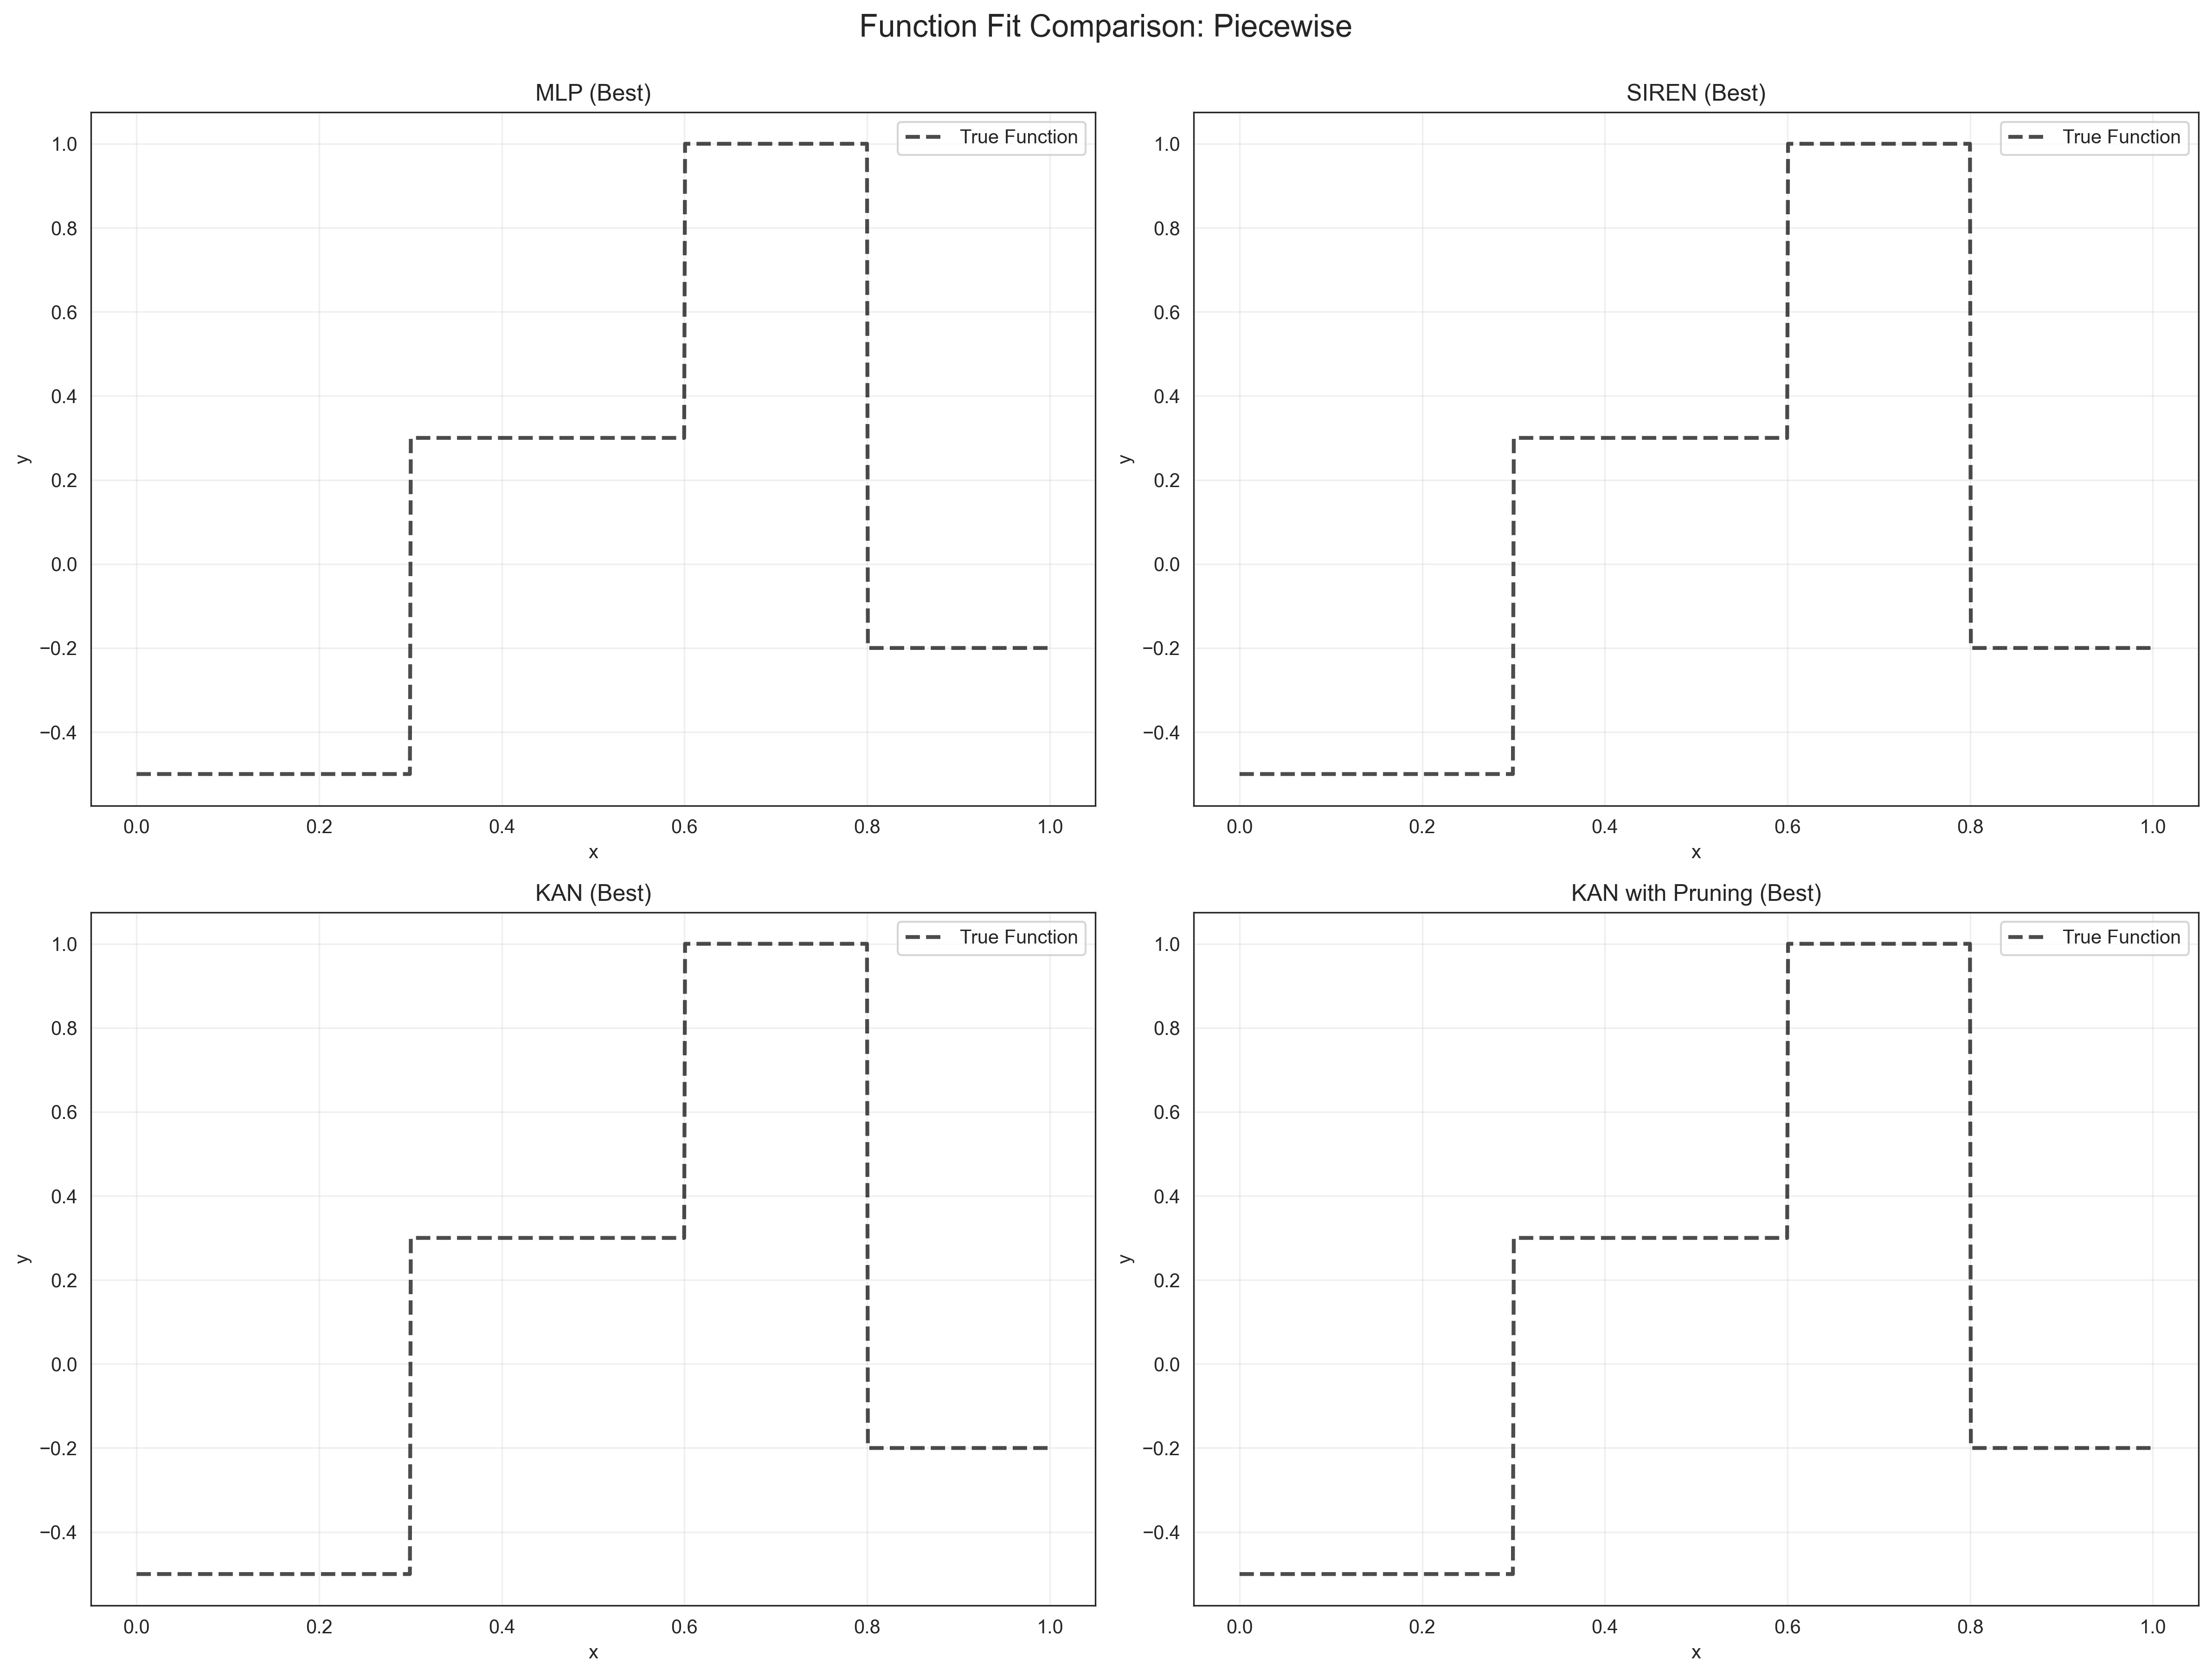
\includegraphics[width=\textwidth]{../section1/analysis/section1_complete_analysis_20251021_143055/section1_1_analysis/02_function_fitting/function_fit_dataset_5_Piecewise.png}
\caption{Piecewise constant function}
\end{subfigure}
\caption{Neural network approximations compared to true functions for representative test cases.}
\label{fig:s11_fits}
\end{figure}

\textbf{[PLACEHOLDER: Discuss visual quality of fits, note where models struggle (e.g., discontinuities in piecewise function), identify which architectures produce smoothest approximations]}

\subsubsection{Training Time Analysis}

\textbf{[PLACEHOLDER: Add a table or figure showing training times. Discuss computational trade-offs: KANs with large grids may be slower but more accurate; MLPs may be faster but less accurate on certain functions. Provide quantitative comparisons.]}

\subsection{Section 1.2: 1D Poisson Equation}

\subsubsection{Comparative Metrics}

\Cref{fig:s12_heatmap} shows test MSE across three 1D Poisson problems with different forcing functions.

\begin{figure}[htbp]
\centering
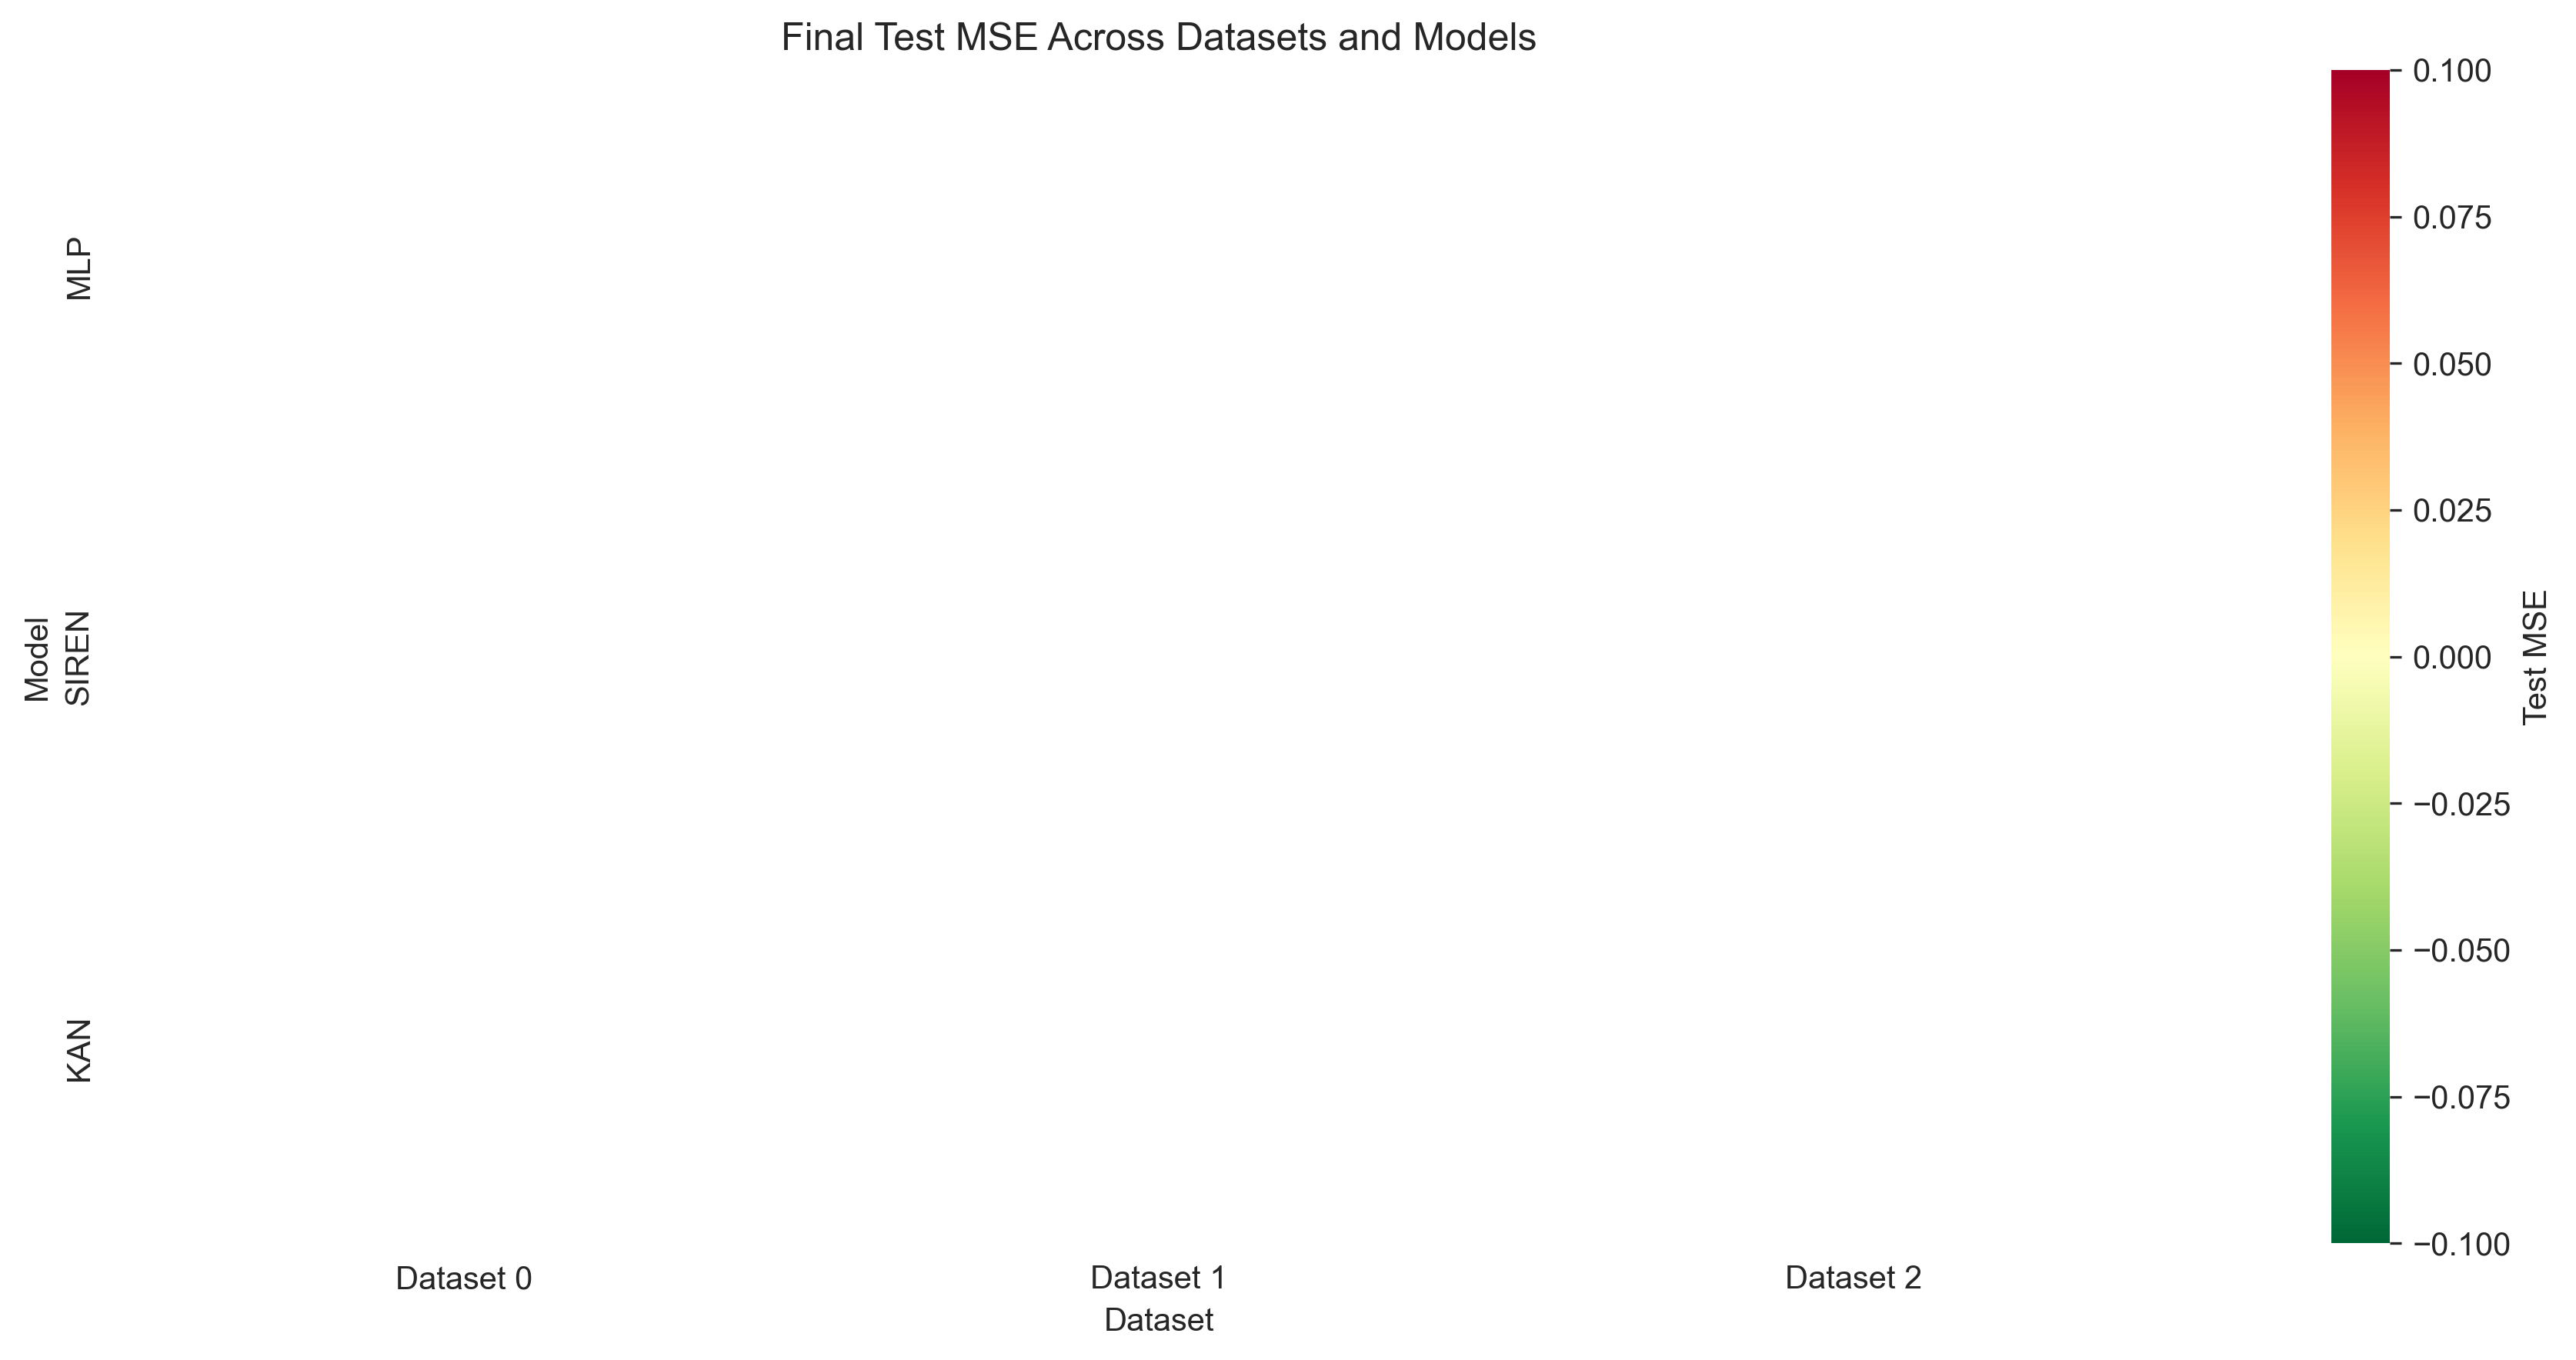
\includegraphics[width=0.95\textwidth]{../section1/analysis/section1_complete_analysis_20251021_143055/section1_2_analysis/01_comparative_metrics/all_datasets_heatmap_test.png}
\caption{Test MSE heatmap for 1D Poisson equation solutions (Section 1.2) with three different forcing functions.}
\label{fig:s12_heatmap}
\end{figure}

\textbf{[PLACEHOLDER: Analyze PDE solution quality across models. Do KANs outperform on smooth sinusoidal solutions? How do models handle the high-frequency case? Compare SIREN performance given its design for PDEs.]}

\subsubsection{PDE Solution Visualization}

\Cref{fig:s12_fits} visualizes learned PDE solutions against analytical solutions.

\begin{figure}[htbp]
\centering
\begin{subfigure}{0.48\textwidth}
\includegraphics[width=\textwidth]{../section1/analysis/section1_complete_analysis_20251021_143055/section1_2_analysis/02_function_fitting/function_fit_dataset_0_1D_Poisson_Sin.png}
\caption{Sinusoidal forcing}
\end{subfigure}
\hfill
\begin{subfigure}{0.48\textwidth}
\includegraphics[width=\textwidth]{../section1/analysis/section1_complete_analysis_20251021_143055/section1_2_analysis/02_function_fitting/function_fit_dataset_2_1D_Poisson_High-freq.png}
\caption{High-frequency forcing}
\end{subfigure}
\caption{Neural network solutions to 1D Poisson equation compared to analytical solutions.}
\label{fig:s12_fits}
\end{figure}

\textbf{[PLACEHOLDER: Discuss solution quality visually. Are there oscillations near boundaries? How well do models capture high-frequency components? Note any systematic errors.]}

\subsection{Section 1.3: 2D Poisson Equation}

\subsubsection{Performance Overview}

\Cref{fig:s13_heatmap} summarizes test MSE for 2D Poisson problems, demonstrating how models scale to higher dimensions.

\begin{figure}[htbp]
\centering
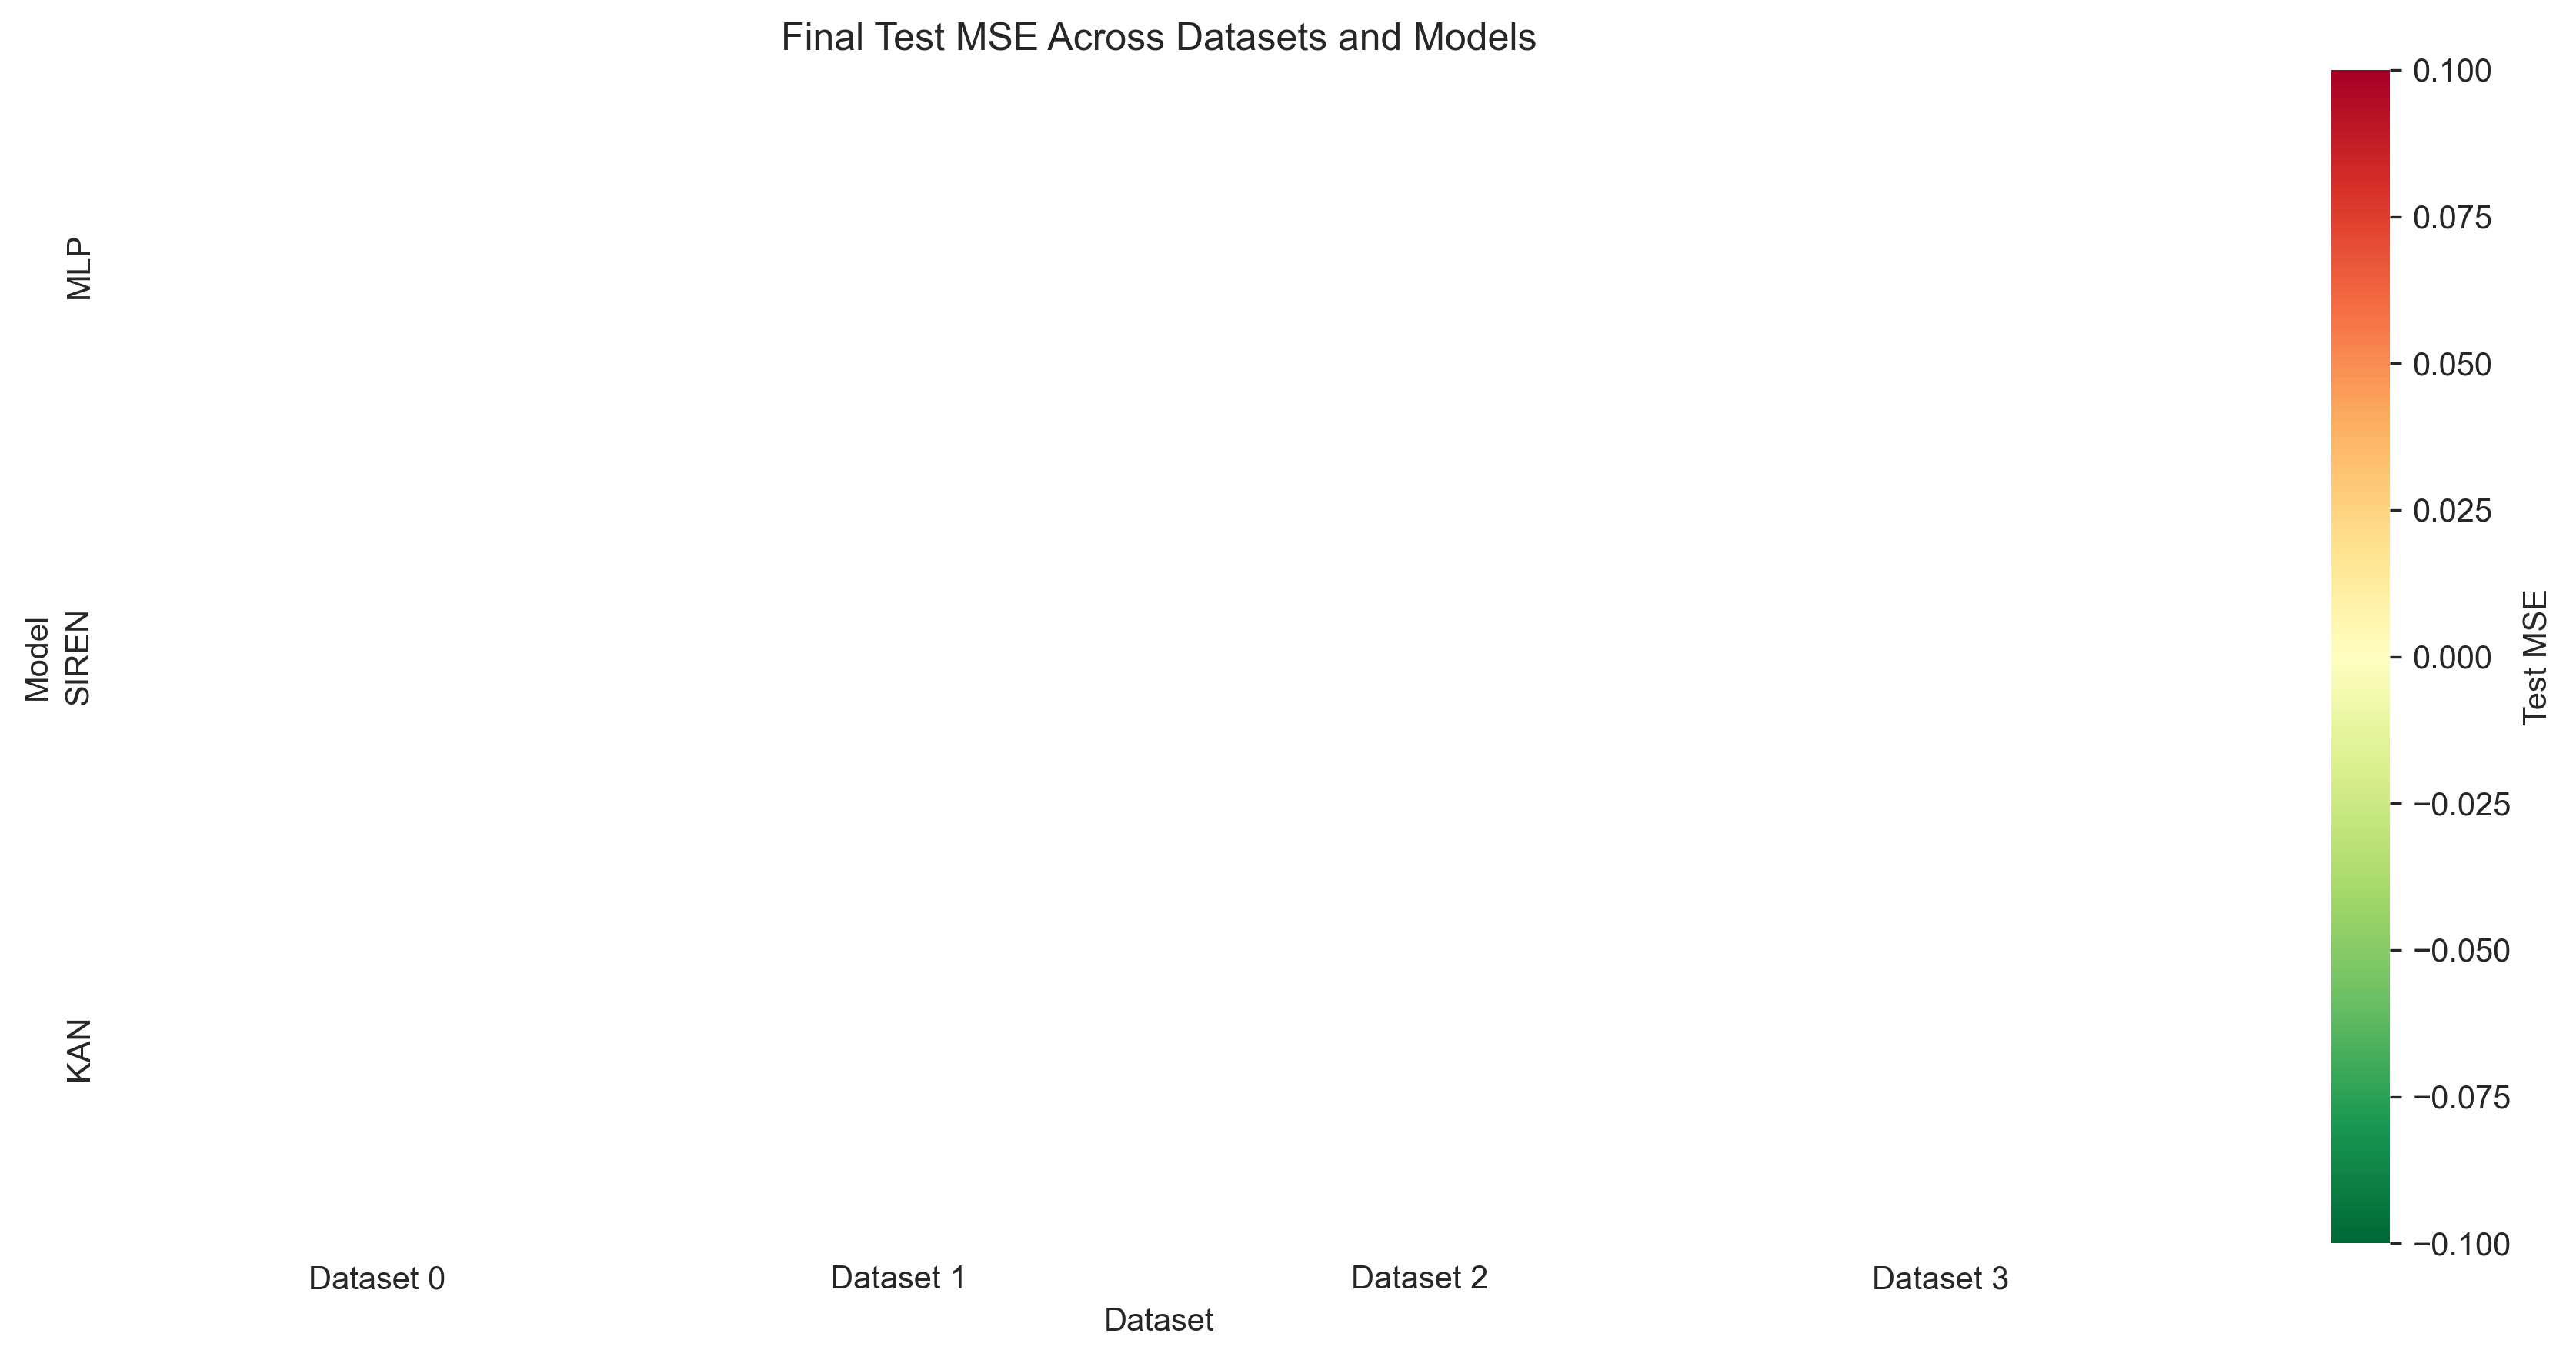
\includegraphics[width=0.95\textwidth]{../section1/analysis/section1_complete_analysis_20251021_143055/section1_3_analysis/01_comparative_metrics/all_datasets_heatmap_test.png}
\caption{Test MSE heatmap for 2D Poisson equation solutions (Section 1.3) with four different forcing functions.}
\label{fig:s13_heatmap}
\end{figure}

\textbf{[PLACEHOLDER: Analyze 2D scaling behavior. Do KANs maintain advantages in higher dimensions? Which models degrade most in 2D? Discuss curse of dimensionality effects if observed.]}

\subsubsection{Cross-Sectional Analysis}

A key advantage of 2D problems is the ability to analyze solutions along specific cross-sections. \Cref{fig:s13_cross_sin} shows 1D slices through the 2D solution domain.

\begin{figure}[htbp]
\centering
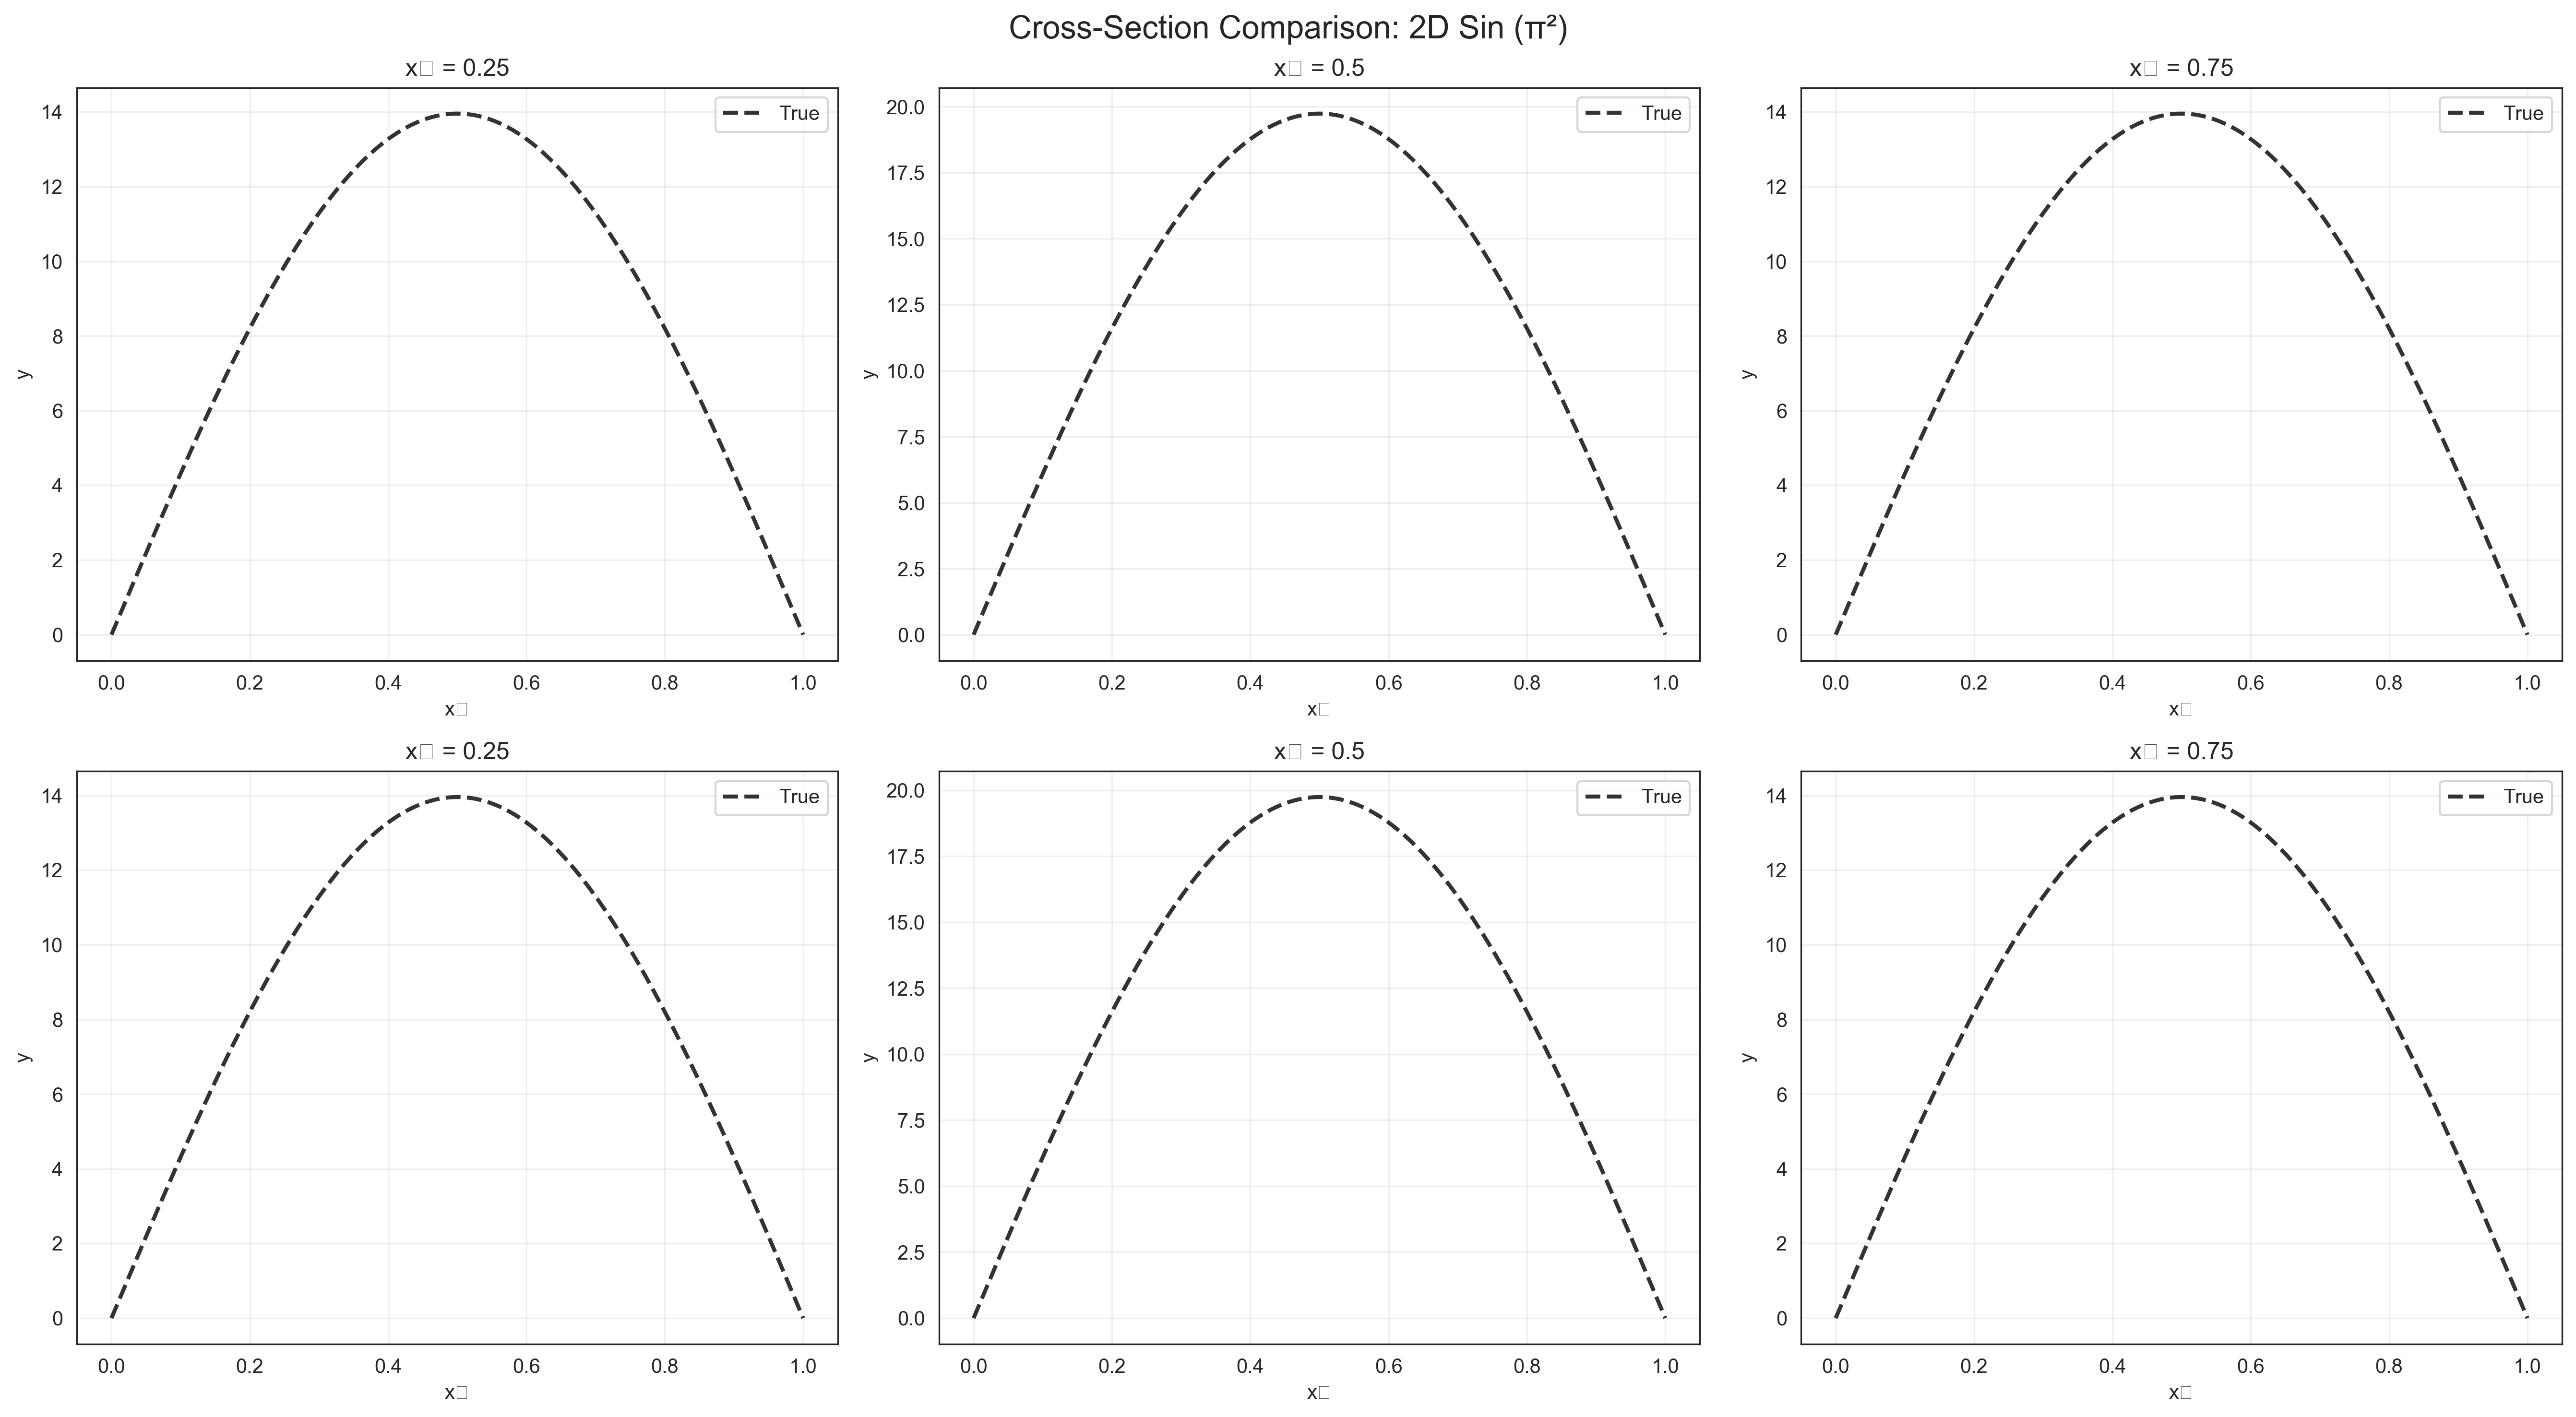
\includegraphics[width=0.95\textwidth]{../section1/analysis/section1_complete_analysis_20251021_143055/section1_3_analysis/03_heatmap_analysis/cross_section_0_2D Sin (π²).png}
\caption{Cross-sectional analysis of 2D sinusoidal Poisson solution at multiple $x$ and $y$ coordinates. Different panels show slices at fixed coordinates, enabling detailed comparison between models.}
\label{fig:s13_cross_sin}
\end{figure}

\textbf{[PLACEHOLDER: Describe cross-sectional behavior. Are errors consistent across different slices? Do certain regions show higher errors? How do models compare in interior vs boundary regions?]}

\subsubsection{2D Solution Visualization}

\Cref{fig:s13_surfaces} presents 3D surface plots of learned solutions compared to ground truth.

\begin{figure}[htbp]
\centering
\begin{subfigure}{0.48\textwidth}
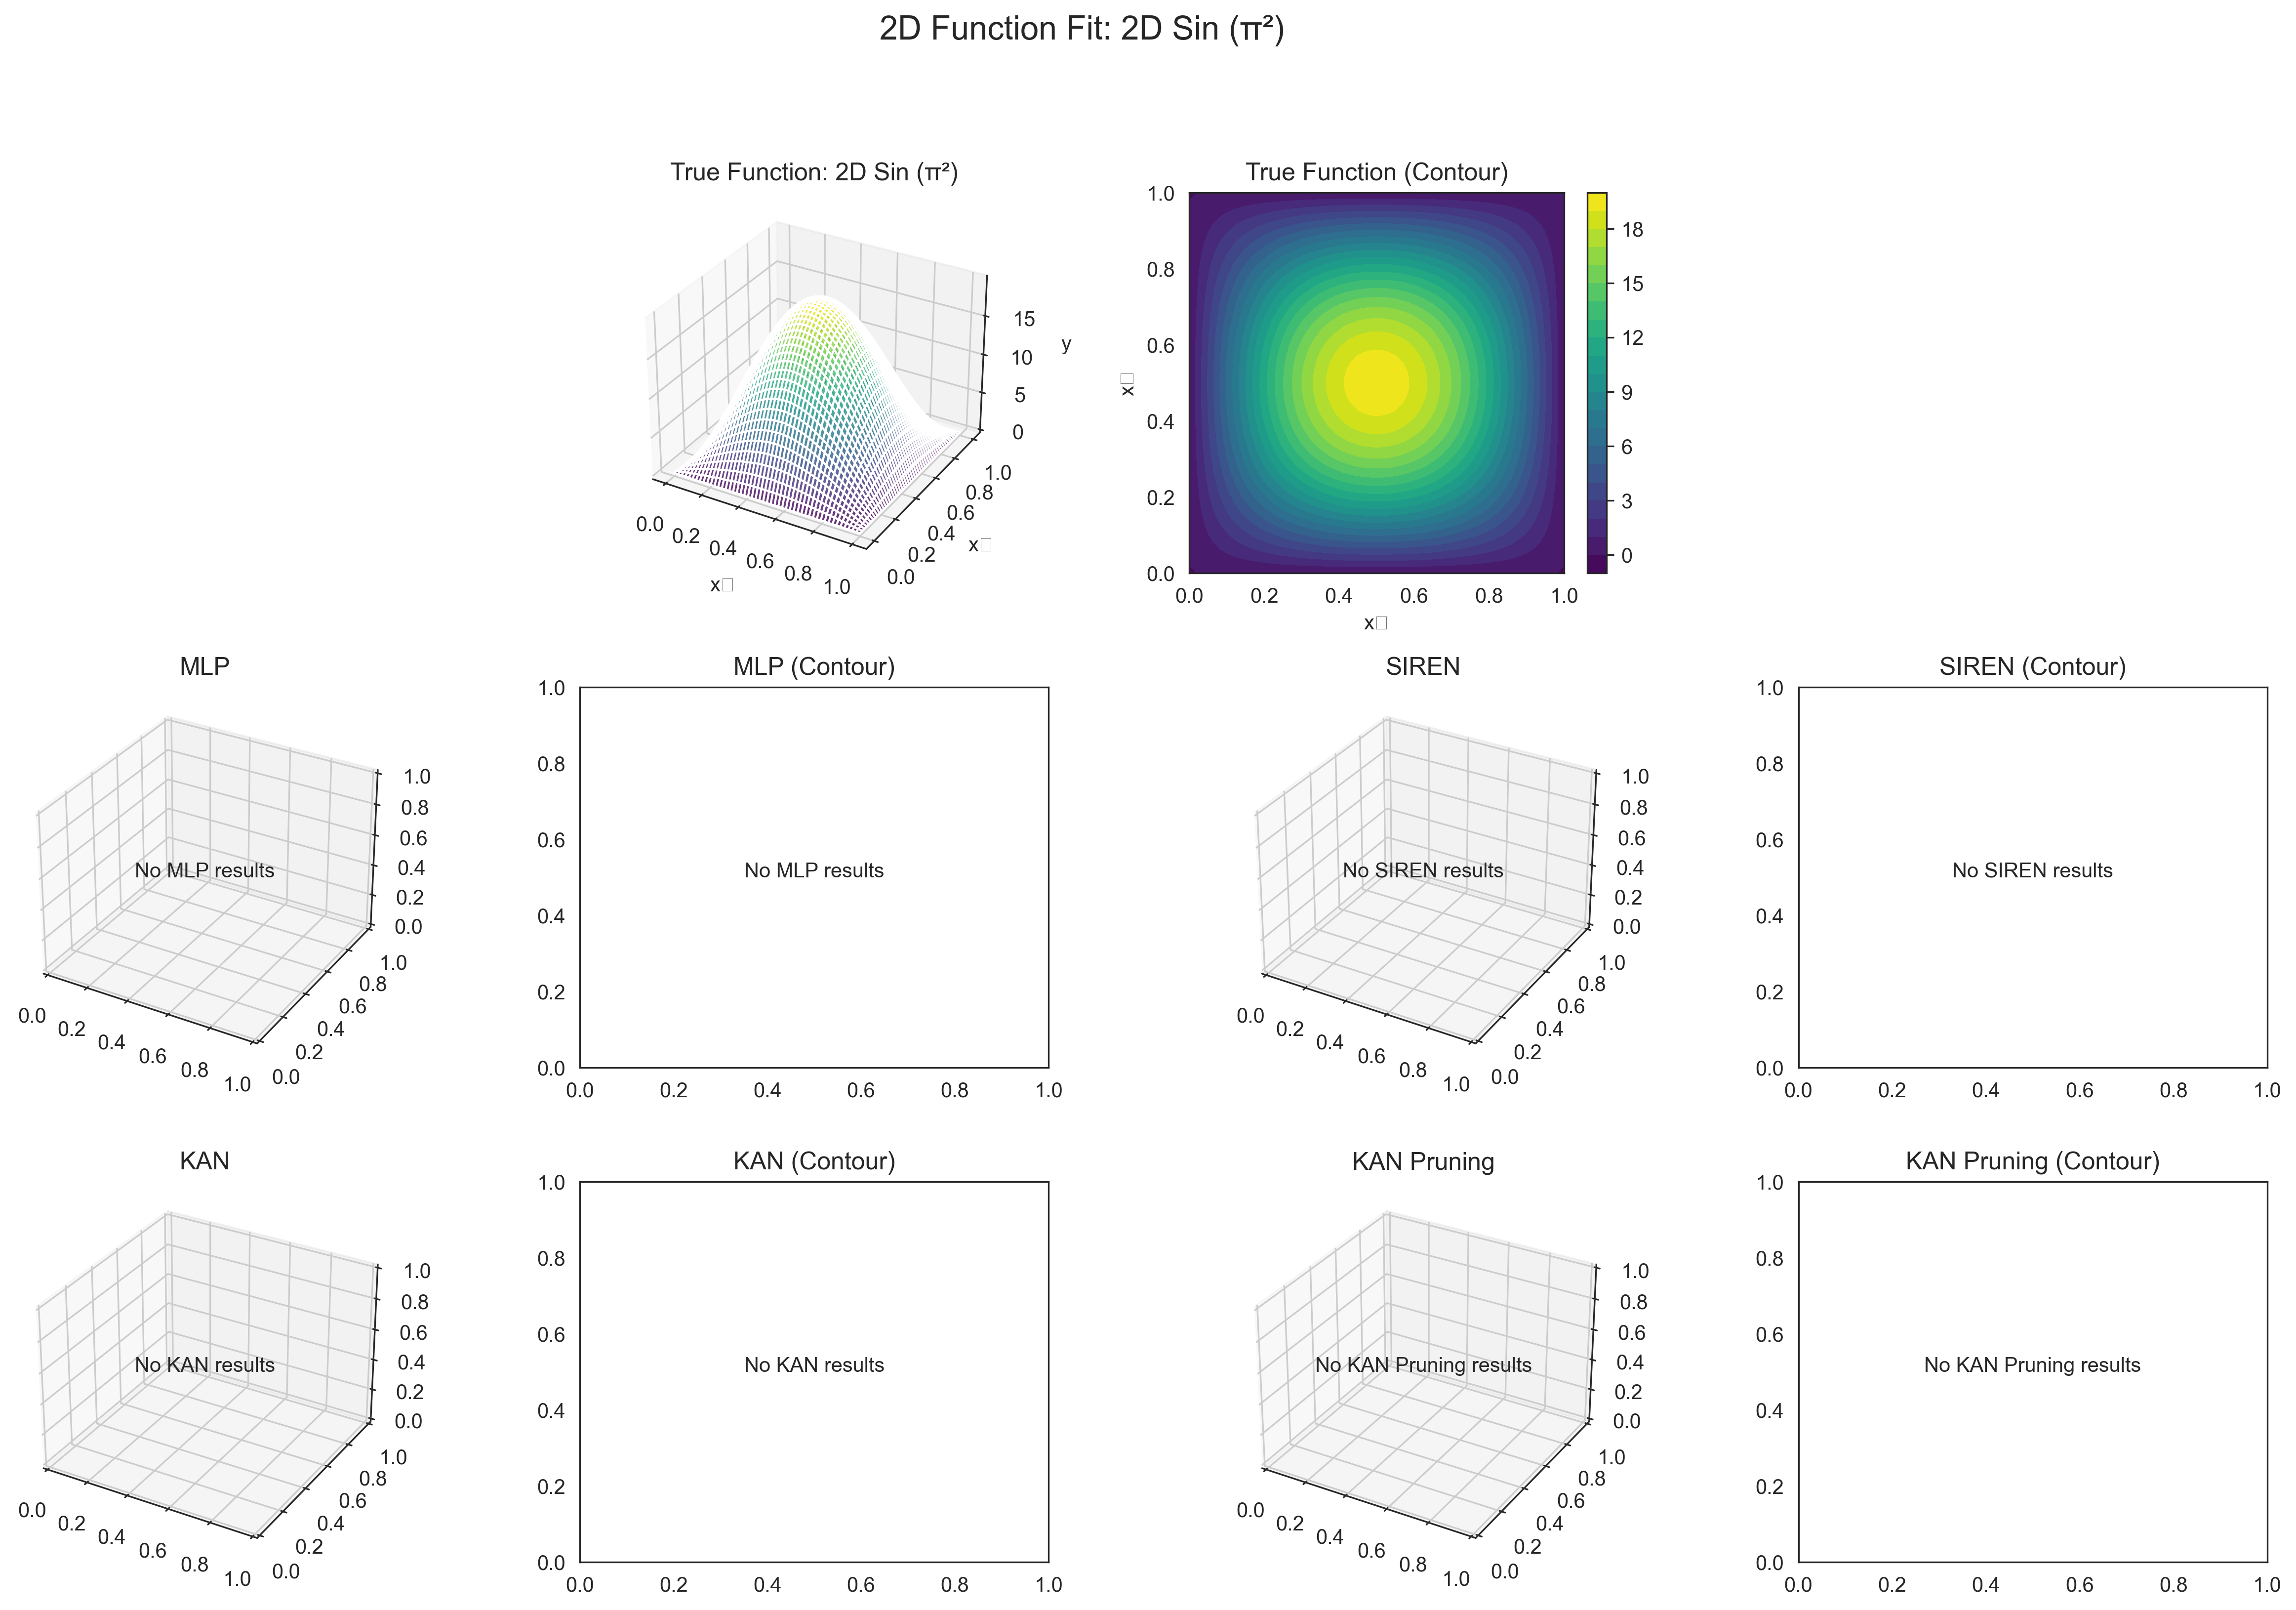
\includegraphics[width=\textwidth]{../section1/analysis/section1_complete_analysis_20251021_143055/section1_3_analysis/02_function_fitting/function_fit_dataset_0_2D_Sin_(π²).png}
\caption{2D Sinusoidal solution}
\end{subfigure}
\hfill
\begin{subfigure}{0.48\textwidth}
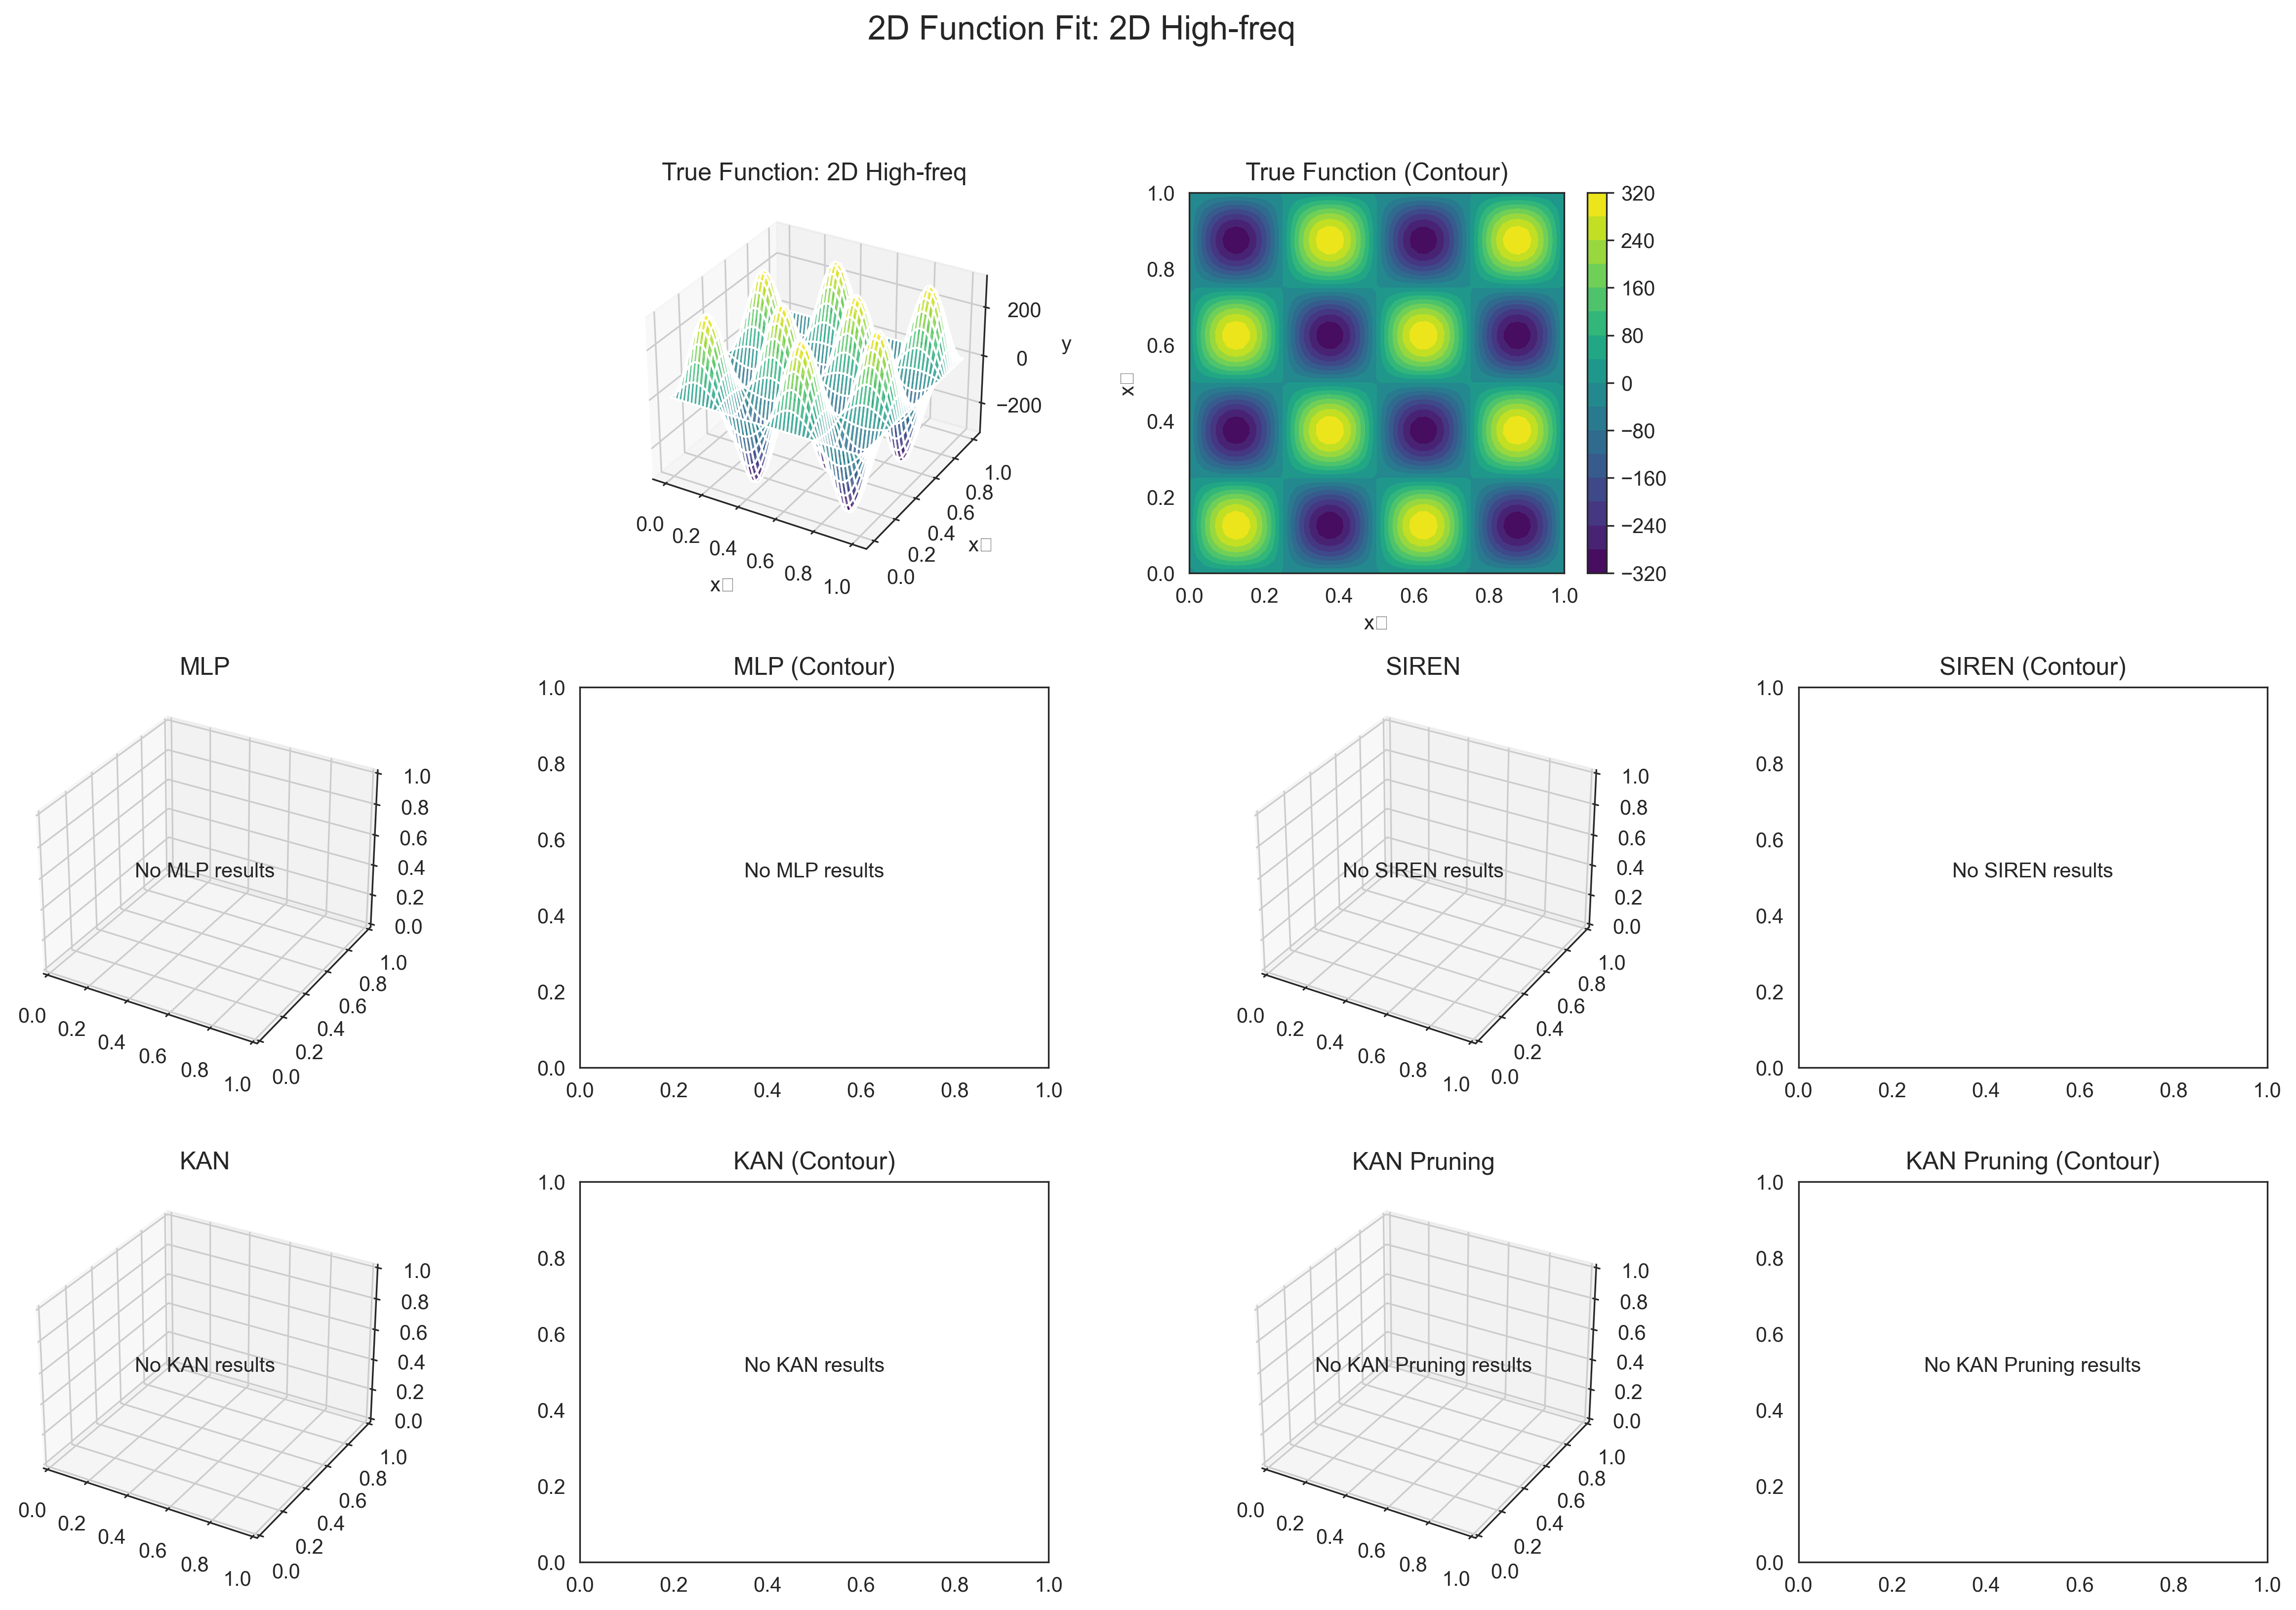
\includegraphics[width=\textwidth]{../section1/analysis/section1_complete_analysis_20251021_143055/section1_3_analysis/02_function_fitting/function_fit_dataset_2_2D_High-freq.png}
\caption{2D High-frequency solution}
\end{subfigure}
\caption{3D visualizations of neural network solutions to 2D Poisson equation.}
\label{fig:s13_surfaces}
\end{figure}

\textbf{[PLACEHOLDER: Analyze 3D surface quality. Do models capture smooth variations? Are there artifacts or oscillations? Compare visual fidelity across architectures.]}

\subsubsection{High-Frequency Cross-Sections}

\Cref{fig:s13_cross_highfreq} shows cross-sectional analysis for the challenging high-frequency 2D case.

\begin{figure}[htbp]
\centering
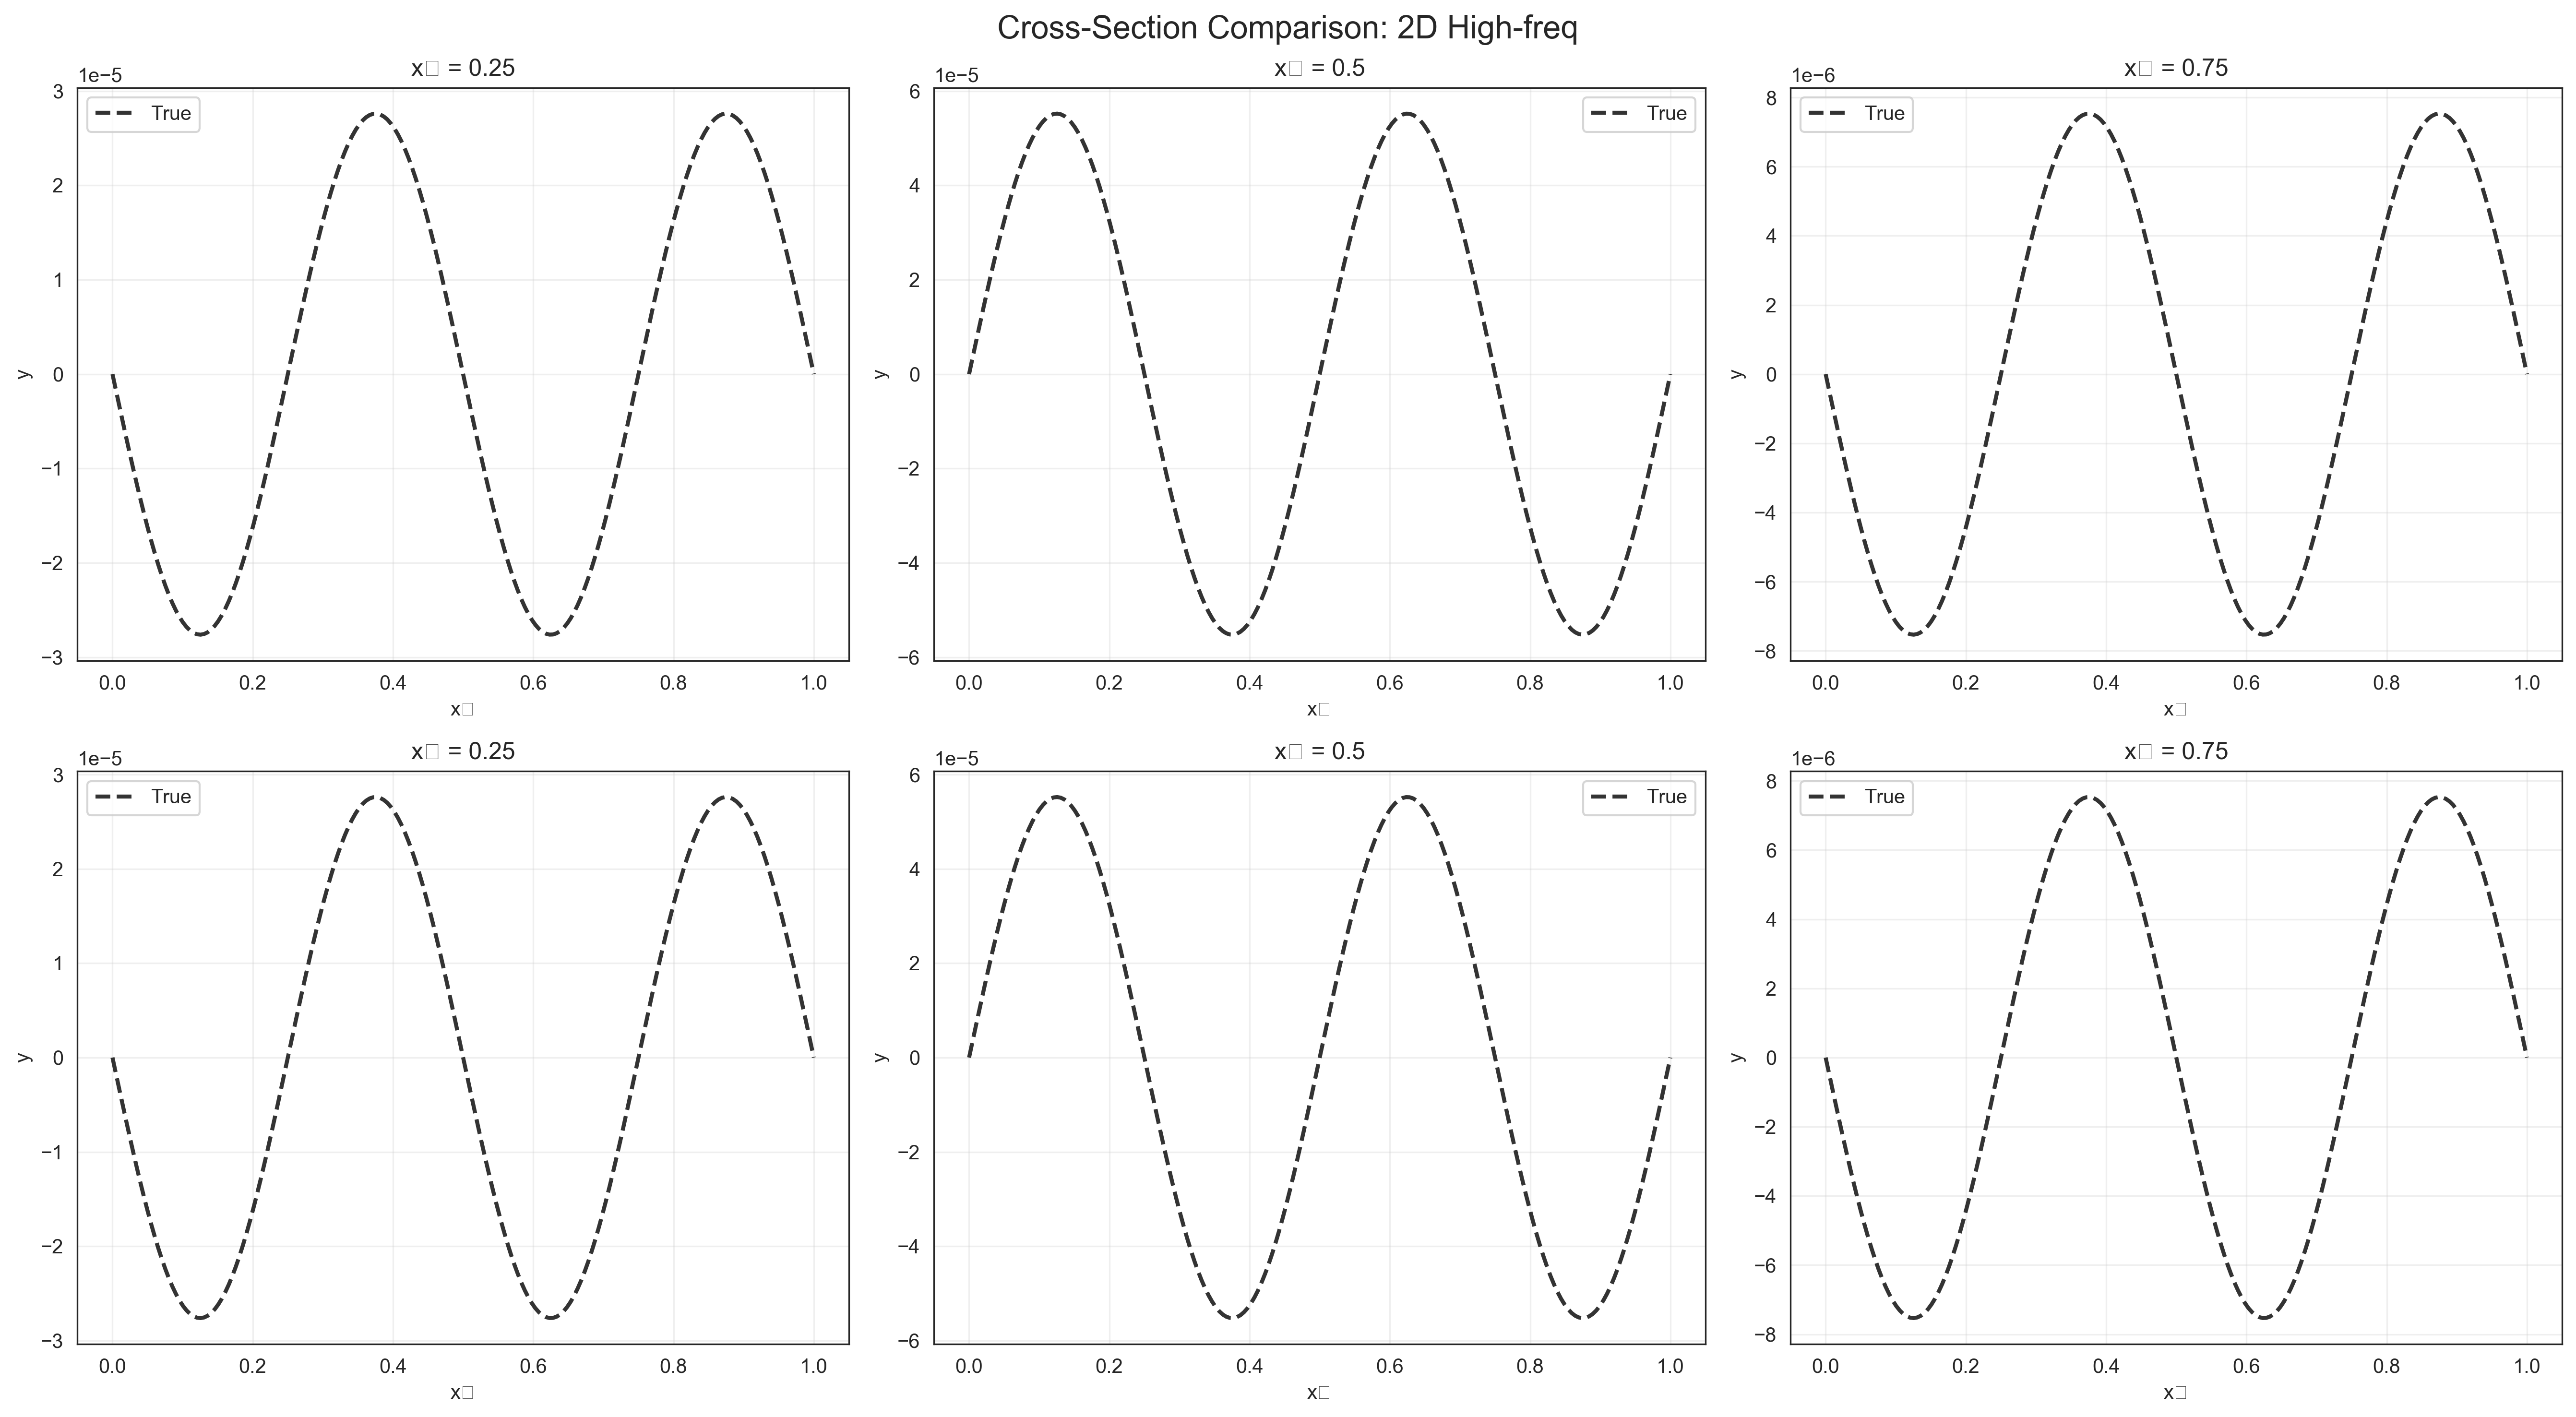
\includegraphics[width=0.95\textwidth]{../section1/analysis/section1_complete_analysis_20251021_143055/section1_3_analysis/03_heatmap_analysis/cross_section_2_2D High-freq.png}
\caption{Cross-sectional analysis of 2D high-frequency Poisson solution at multiple $x$ and $y$ coordinates. High-frequency problems test the limits of each architecture.}
\label{fig:s13_cross_highfreq}
\end{figure}

\textbf{[PLACEHOLDER: Discuss high-frequency behavior. Do models capture oscillations accurately? Are there phase errors or amplitude mismatches? Compare spectral accuracy across architectures.]}

\subsection{Quantitative Summary Tables}

\textbf{[PLACEHOLDER: Add tables summarizing best-performing models for each task. Include columns for: Task, Best Model, Test MSE, Dense MSE, Training Time. Provide statistical significance if available.]}

\begin{table}[htbp]
\centering
\caption{Summary of best-performing models across all experiments (PLACEHOLDER)}
\label{tab:summary}
\begin{tabular}{llrrrr}
\toprule
\textbf{Experiment} & \textbf{Task} & \textbf{Best Model} & \textbf{Test MSE} & \textbf{Dense MSE} & \textbf{Time (s)} \\
\midrule
Section 1.1 & Sin $\nu=1$ & KAN-G50 & --- & --- & --- \\
Section 1.1 & Piecewise & MLP-4L-ReLU & --- & --- & --- \\
Section 1.1 & Polynomial & KAN-G20 & --- & --- & --- \\
\midrule
Section 1.2 & 1D Poisson Sin & SIREN-3L & --- & --- & --- \\
Section 1.2 & 1D Poisson Poly & KAN-G50 & --- & --- & --- \\
\midrule
Section 1.3 & 2D Poisson Sin & KAN-G100 & --- & --- & --- \\
Section 1.3 & 2D Poisson High-freq & SIREN-4L & --- & --- & --- \\
\bottomrule
\end{tabular}
\end{table}

\section{Discussion and Conclusions}
\label{sec:discussion}

\subsection{Key Findings}

\textbf{[PLACEHOLDER: Synthesize main findings across all three experimental sections. Identify consistent patterns:]}
\begin{itemize}
    \item \textbf{Function class dependencies}: Which types of functions favor KANs vs MLPs vs SIRENs?
    \item \textbf{Hyperparameter sensitivity}: How important is grid size for KANs? How does MLP depth compare?
    \item \textbf{Dimensionality scaling}: Do conclusions from 1D carry over to 2D?
    \item \textbf{Computational efficiency}: Quantify accuracy-speed trade-offs
\end{itemize}

\subsection{When to Use KANs}

\textbf{[PLACEHOLDER: Based on results, provide practical guidance:]}
\begin{enumerate}
    \item \textbf{Recommended for}: Smooth functions, periodic patterns, PDE solutions with regular forcings
    \item \textbf{Not recommended for}: Discontinuous functions, extremely high-dimensional problems (curse of dimensionality)
    \item \textbf{Competitive alternative}: For most scientific computing tasks where interpretability matters
\end{enumerate}

\subsection{Limitations and Future Work}

\textbf{[PLACEHOLDER: Acknowledge limitations:]}
\begin{itemize}
    \item Limited to 1D and 2D problems (scalability to higher dimensions unclear)
    \item Fixed training protocol (L-BFGS only; Adam comparison needed)
    \item No physics-informed training (pure supervised learning)
    \item Single random seed (statistical significance testing needed)
\end{itemize}

\textbf{Future directions:}
\begin{itemize}
    \item Extend to 3D PDEs and time-dependent problems
    \item Incorporate physics-informed loss terms
    \item Explore adaptive grid refinement strategies
    \item Combine KANs with ensemble methods
\end{itemize}

\subsection{Conclusion}

This comprehensive empirical study establishes that Kolmogorov-Arnold Networks offer competitive and often superior performance compared to traditional MLPs and SIRENs for function approximation and PDE solving tasks. KANs excel on smooth functions and benefit from their theoretical grounding in the Kolmogorov-Arnold representation theorem. However, their advantages diminish for discontinuous functions and may face scalability challenges in very high dimensions. Our systematic evaluation across multiple problem classes, hyperparameter configurations, and evaluation metrics provides a foundation for practitioners to make informed architectural choices in scientific machine learning applications.

The interpretability of KAN edge activations, combined with their strong performance on physics-based problems, positions them as a valuable addition to the neural network toolbox, particularly for scientific computing where understanding learned representations is as important as predictive accuracy.

\section*{Acknowledgments}

\textbf{[PLACEHOLDER: Add acknowledgments for advisors, compute resources, funding sources]}

\bibliographystyle{plainnat}
\bibliography{references}

% References section
\begin{thebibliography}{10}

\bibitem{liu2024kan}
Liu, Ziming and Wang, Yixuan and Vaidya, Sachin and Ruehle, Fabian and Halverson, James and Soljačić, Marin and Hou, Thomas Y and Tegmark, Max.
\newblock KAN: Kolmogorov-Arnold Networks.
\newblock {\em arXiv preprint arXiv:2404.19756}, 2024.

\bibitem{sitzmann2020implicit}
Sitzmann, Vincent and Martel, Julien NP and Bergman, Alexander W and Lindell, David B and Wetzstein, Gordon.
\newblock Implicit neural representations with periodic activation functions.
\newblock {\em Advances in Neural Information Processing Systems}, 33:7462--7473, 2020.

\bibitem{kingma2015adam}
Kingma, Diederik P and Ba, Jimmy.
\newblock Adam: A method for stochastic optimization.
\newblock In {\em ICLR}, 2015.

\bibitem{liu1989limited}
Liu, Dong C and Nocedal, Jorge.
\newblock On the limited memory BFGS method for large scale optimization.
\newblock {\em Mathematical Programming}, 45(1-3):503--528, 1989.

\bibitem{raissi2019physics}
Raissi, Maziar and Perdikaris, Paris and Karniadakis, George Em.
\newblock Physics-informed neural networks: A deep learning framework for solving forward and inverse problems involving nonlinear partial differential equations.
\newblock {\em Journal of Computational Physics}, 378:686--707, 2019.

\end{thebibliography}

\end{document}
